% file thesis.tex
% Archivo thesis.tex
% Documento maestro que incluye todos los paquetes necesarios para el documento
% principal.

% Documento obtenido por un sinfin de iteraciones de administradores del LDC
% Estructura actual hecha por:
% Jairo Lopez <jairo@ldc.usb.ve>
% Actualizado ligeramente por:
% Alexander Tough 

\documentclass[oneside,12pt,letterpaper]{report}
\tolerance=1000  
\hbadness=10000  
\raggedbottom

% Para escribir algoritmos
\usepackage{listings}
\usepackage{algpseudocode}
\usepackage{algorithmicx}
\usepackage{algorithm}

% Paquetes para manejar graficos
\usepackage{epsf}
\usepackage[pdftex]{graphicx}
\usepackage{epsfig}
% Simbolos matematicos
\usepackage{latexsym,amssymb}
% Paquetes para presentar una tesis decente.
\usepackage{setspace,cite} % Doble espacio para texto, espacio singular para
                           % los caption y pie de pagina
\usepackage[table]{xcolor}
\usepackage{tikz}
\usepackage[T1]{fontenc}

\usetikzlibrary{shapes.geometric,arrows}

\usetikzlibrary{arrows,shapes}
\usepackage{verbatim}

\usepackage{comment}

% Paquetes no utilizados para citas
%\usepackage{mcite} 
%\usepackage{draft} 

\usepackage{wrapfig}
\usepackage{alltt}

% Acentos 
\usepackage[spanish,activeacute,es-noquoting]{babel}

\usepackage[spanish]{translator}
\usepackage[utf8]{inputenc}
\usepackage{color, xcolor, colortbl}
\usepackage{multirow}
\usepackage{subfig}
\usepackage[OT1]{fontenc}
\usepackage{tocbibind}
\usepackage{anysize}
\usepackage{listings} 

% Para poder tener texto asiatico
%\usepackage{CJK}

% Opciones para los glosarios
\usepackage[style=altlist,toc,numberline,acronym]{glossaries}
\usepackage{url}
\usepackage{amsthm}
\usepackage{amsmath}
\usepackage{fancyhdr} % Necesario para los encabezados
\usepackage{fancyvrb}
\usepackage{makeidx} % En caso de necesitar indices.
\makeindex  % Necesitado para los indices

% Definiciones para definicions, teoremas y lemas
\theoremstyle{definition} \newtheorem{definicion}{Definici\'{o}n}
\theoremstyle{plain} \newtheorem{teorema}{Teorema}
\theoremstyle{plain} \newtheorem{lema}{Lema}

% Para la creacion de los pdfs
\usepackage{hyperref}

% Para resolver el lio del Unicode para la informacion de los PDFs
% En pdftitle coloca el nombre de su proyecto de grado/pasantia.
% En pdfauthor coloca su nombre.
\hypersetup{
    pdftitle = {Desarrollo de un prototipo de robot humanoide que busque, encuentre y patee una pelota },
    pdfauthor={Jennifer Dos Reis y Juliana Leon},
    colorlinks,
    citecolor=black,
    filecolor=black,
    linkcolor=black,
    urlcolor=black,
    backref,
    pdftex
}

\definecolor{brown}{rgb}{0.7,0.2,0}
\definecolor{darkgreen}{rgb}{0,0.6,0.1}
\definecolor{darkgrey}{rgb}{0.4,0.4,0.4}
\definecolor{lightgrey}{rgb}{0.95,0.95,0.95}

\usepackage{listings}
\lstnewenvironment{code}{\lstset{basicstyle=\small}}{}

\lstset{escapeinside=~~}
\lstset{
   frame=single,
   framerule=1pt,
   showstringspaces=false,
   basicstyle=\footnotesize\ttfamily,
   keywordstyle=\textbf,
   backgroundcolor=\color{lightgrey}
}

% Crea el glosario
\makeglossaries

% Incluye el glosario
\newglossaryentry{C++}
{
  name=C++,
  description={Es un lenguaje de programaci\'on imperativo y orientado a objetos.}
}
\newglossaryentry{AVR}
{
  name=AVR,
  description={Es una familia de microcontroladores de instrucciones reducidas de la compañía Atmel.}
}

\newglossaryentry{framework}
{
  name=framework,
  description={(Marco de trabajo) Es un conjunto de técnicas, conceptos y estilos de trabajo que se establecen para resolver un problema particular y que sirve de referencia para solucionar problemas similares.}
}

\newglossaryentry{TightVNC}
{
  name=TightVNC,
  description={Es un paquete de software que sirve para controlar la interfaz gráfica  de ordenadores remotos.}
}

\newglossaryentry{IDE}
{
  name=IDE,
  description={(Integrated development environment / Entorno de desarrollo integrado): Es un programa diseñado para facilitar la programación en uno o varios lenguajes. Usualmente incluye herramientas de compilación, editor de textos y depurador.}
}

\newglossaryentry{ROS}
{
  name=ROS,
  description={(Robot Operating System / Sistema de operación para robots ): Es un framework que provee herramientas para ayudar a desarrolladores de aplicaciones para robots.}
}

\newglossaryentry{BSD}
{
  name=Licencia BSD,
  description={(Berkeley Software Distribution / distribución de software berkeley) : Es una licencia para software libre otorgada principalmente a sistemas BSD.}
}

\newglossaryentry{XBEE}
{
  name=XBEE,
  description={Es una familia de módulos de radio, con protocolo de comunicación inalámbrica basado en radio frecuencias.}
}

\newglossaryentry{CSI}
{
  name=CSI,
  description={(Camera Serial Interface / Interfaz serial para cámaras ): Es un estándar que define la interfaz de comunicación entre una cámara y un procesador. Es comúnmente utilizado en dispositivos móviles.}
}
     
\newglossaryentry{MMAL}
{
  name=MMAL,
  description={(Multi-Media Abstraction Layer / Capa de abstracción multimedia): Es una librería que brinda una interfaz de bajo nivel para controlar dispositivos que se ejecutan en el núcleo de video de la Raspberry Pi, como el módulo de cámara.}
}
 
\newglossaryentry{V4L}
{
  name=V4L,
  description={(Video 4 Linux / video para linux): Es una interfaz de programación de video para Linux. Uno de los tipos de dispositivos soportados son las cámaras web USB.}
}

\newglossaryentry{BGR}
{
  name=BGR,
  description={(Red Green Blue / rojo, verde, azul): Es un modelo de color que se basa en la intensidad de los colores primarios de la luz (rojo, verde y azul).}
}
  
\newglossaryentry{HSV}
{
  name=HSV,
  description={(Hue, Saturation, Value / Matiz, Saturación, Valor): Es un modelo de color que se basa en las cualidades de matiz, saturación y valor del color.}
}

\newglossaryentry{HDMI}
{
  name=HDMI,
  description={(High-Definition Multimedia Interface/ interfaz multimedia de alta definición): Es una interfaz para transferir datos de audio y video digital entre un dispositivo y un monitor, proyector, televisor digital o dispositivo de audio digital.}
}

\newglossaryentry{SD}
{
  name=SD,
  description={(Secure Digital / Digital Seguro) : Es un formato de tarjetas de memoria de almacenamiento digital. Existen tarjetas SD con diferentes características en cuanto su clase, capacidad de almacenamiento y tamaño físico.}
}  

\newglossaryentry{LEGO}
{
  name=LEGO,
  description={ Es una serie de juguetes de construcci\'on, que ofrece um kit de materiales para rob\'otica llamada Mindstorms. La serie posee una trajeta programable, sensores y actuadores}
}  

\newglossaryentry{DC}
{
  name=Motor DC,
  description={ Es un motor de corriente directa que transforma la energ\'ia el\'ectrica en mec\'anica generando un movimiento rotatorio}
}  

\newglossaryentry{USB}
{
  name=USB,
  description={(Universal Serial Bus): Es un bus est\'andar de conecci\'on, comunicaci\'on y fuente de poder entre dispositivos electr\'onicos}
}  


\newglossaryentry{UART}
{
  name=UART,
  description={(Universal Asynchronous Receiver/Transmitter): Es dispositivo para la comunicaci\'on est\'andar as\'incrona. }
}  

\newglossaryentry{VGA}
{
  name=VGA,
  description={(Video Graphics Array): Es un conector de video est\'andar, una interfaz de video usada para proyectar video en alta defini\'on }
}  

\newglossaryentry{raspivid}
{
  name=Raspivid,
  description={ Es una herramienta de captura de video por medio de comandos en la Raspeberry Pi}
} 

\newglossaryentry{raspistill}
{
  name=Raspistill,
  description={ Es una herramienta de captura de fotos por l\'inea de comandos en la Raspberry Pi }
} 


% Para crear la hoja escaneada de las firmas
\usepackage[absolute]{textpos}

% Pone los nombres y las opciones para mostrar los codigos fuentes
\lstset{language=C, breaklines=true, frame=single, showstringspaces=false,
        showtabs=false, numbers=left, keywordstyle=\color{black},
        basicstyle=\footnotesize, captionpos=b }
\renewcommand{\lstlistingname}{C\'{o}digo fuente}
\renewcommand{\lstlistlistingname}{\'{I}ndice de c\'{o}digos fuentes}

\newcommand{\todo}{ TODO: }

% Dimensiones de la pagina
\setlength{\headheight}{15pt}
\marginsize{3cm}{2cm}{2cm}{2cm}

%%%%%%%%%%%%%%%%%%%%%%%%%%%%%%%%%%%%%%%%%%%%%%%%%%%%%%%%%%%%%%%%%%%%%%%%%%%
%%%%%%%%%%%%%%%%      end of preamble and start of document     %%%%%%%%%%%
%%%%%%%%%%%%%%%%%%%%%%%%%%%%%%%%%%%%%%%%%%%%%%%%%%%%%%%%%%%%%%%%%%%%%%%%%%%
\begin{document}

% Pagina de titulo
% Pagina de titulo
\begin{titlepage}
\begin{center}

% Upper part (aqui ya esta incluido el logo de la USB).

\includegraphics[scale=0.5,type=png,ext=.png,read=.png]{imagenes/cebolla} \\

% Encabezado
\textsc {\large UNIVERSIDAD SIMÓN BOLÍVAR} \\
\textsc{\bfseries DECANATO DE ESTUDIOS PROFESIONALES\\
COORDINACI'ON DE INGENIER'IA DE LA COMPUTACI'ON}

\bigskip
\bigskip
\bigskip
\bigskip
\bigskip
\bigskip
\bigskip
\bigskip
\bigskip

% Title/Titulo
% Aqui ponga el nombre de su proyecto de grado/pasantia larga
\textsc{\bfseries Desarrollo de un prototipo de robot humanoide que busque, encuentre y patee una pelota de forma autónoma e inteligente}

\bigskip
\bigskip
\bigskip
\bigskip
\bigskip

% Author and supervisor/Autor y tutor
\begin{minipage}{\textwidth}
\centering
Por: \\
Jennifer Dos Reis De Nóbrega \\ Juliana Le\'on Quinteiro\\

\bigskip
\bigskip
\bigskip

Realizado con la asesoría de: \\
Ivette Carolina Mart\'inez 
\end{minipage}

\bigskip
\bigskip
\bigskip
\bigskip
\bigskip
\bigskip
\bigskip
\bigskip
\bigskip

% Bottom half
{PROYECTO DE GRADO \\ Presentado ante la Ilustre Universidad Simón Bolívar \\
como requisito parcial para optar al título de \\ Ingeniero en Computación} \\

\bigskip
\bigskip
\vfill

% Date/Fecha 
{\large \bfseries Sartenejas, 
%FECHA
Noviembre 2014}

\end{center}
\end{titlepage}


% Pagina de acta final (vacio)
%\pagestyle{empty}
%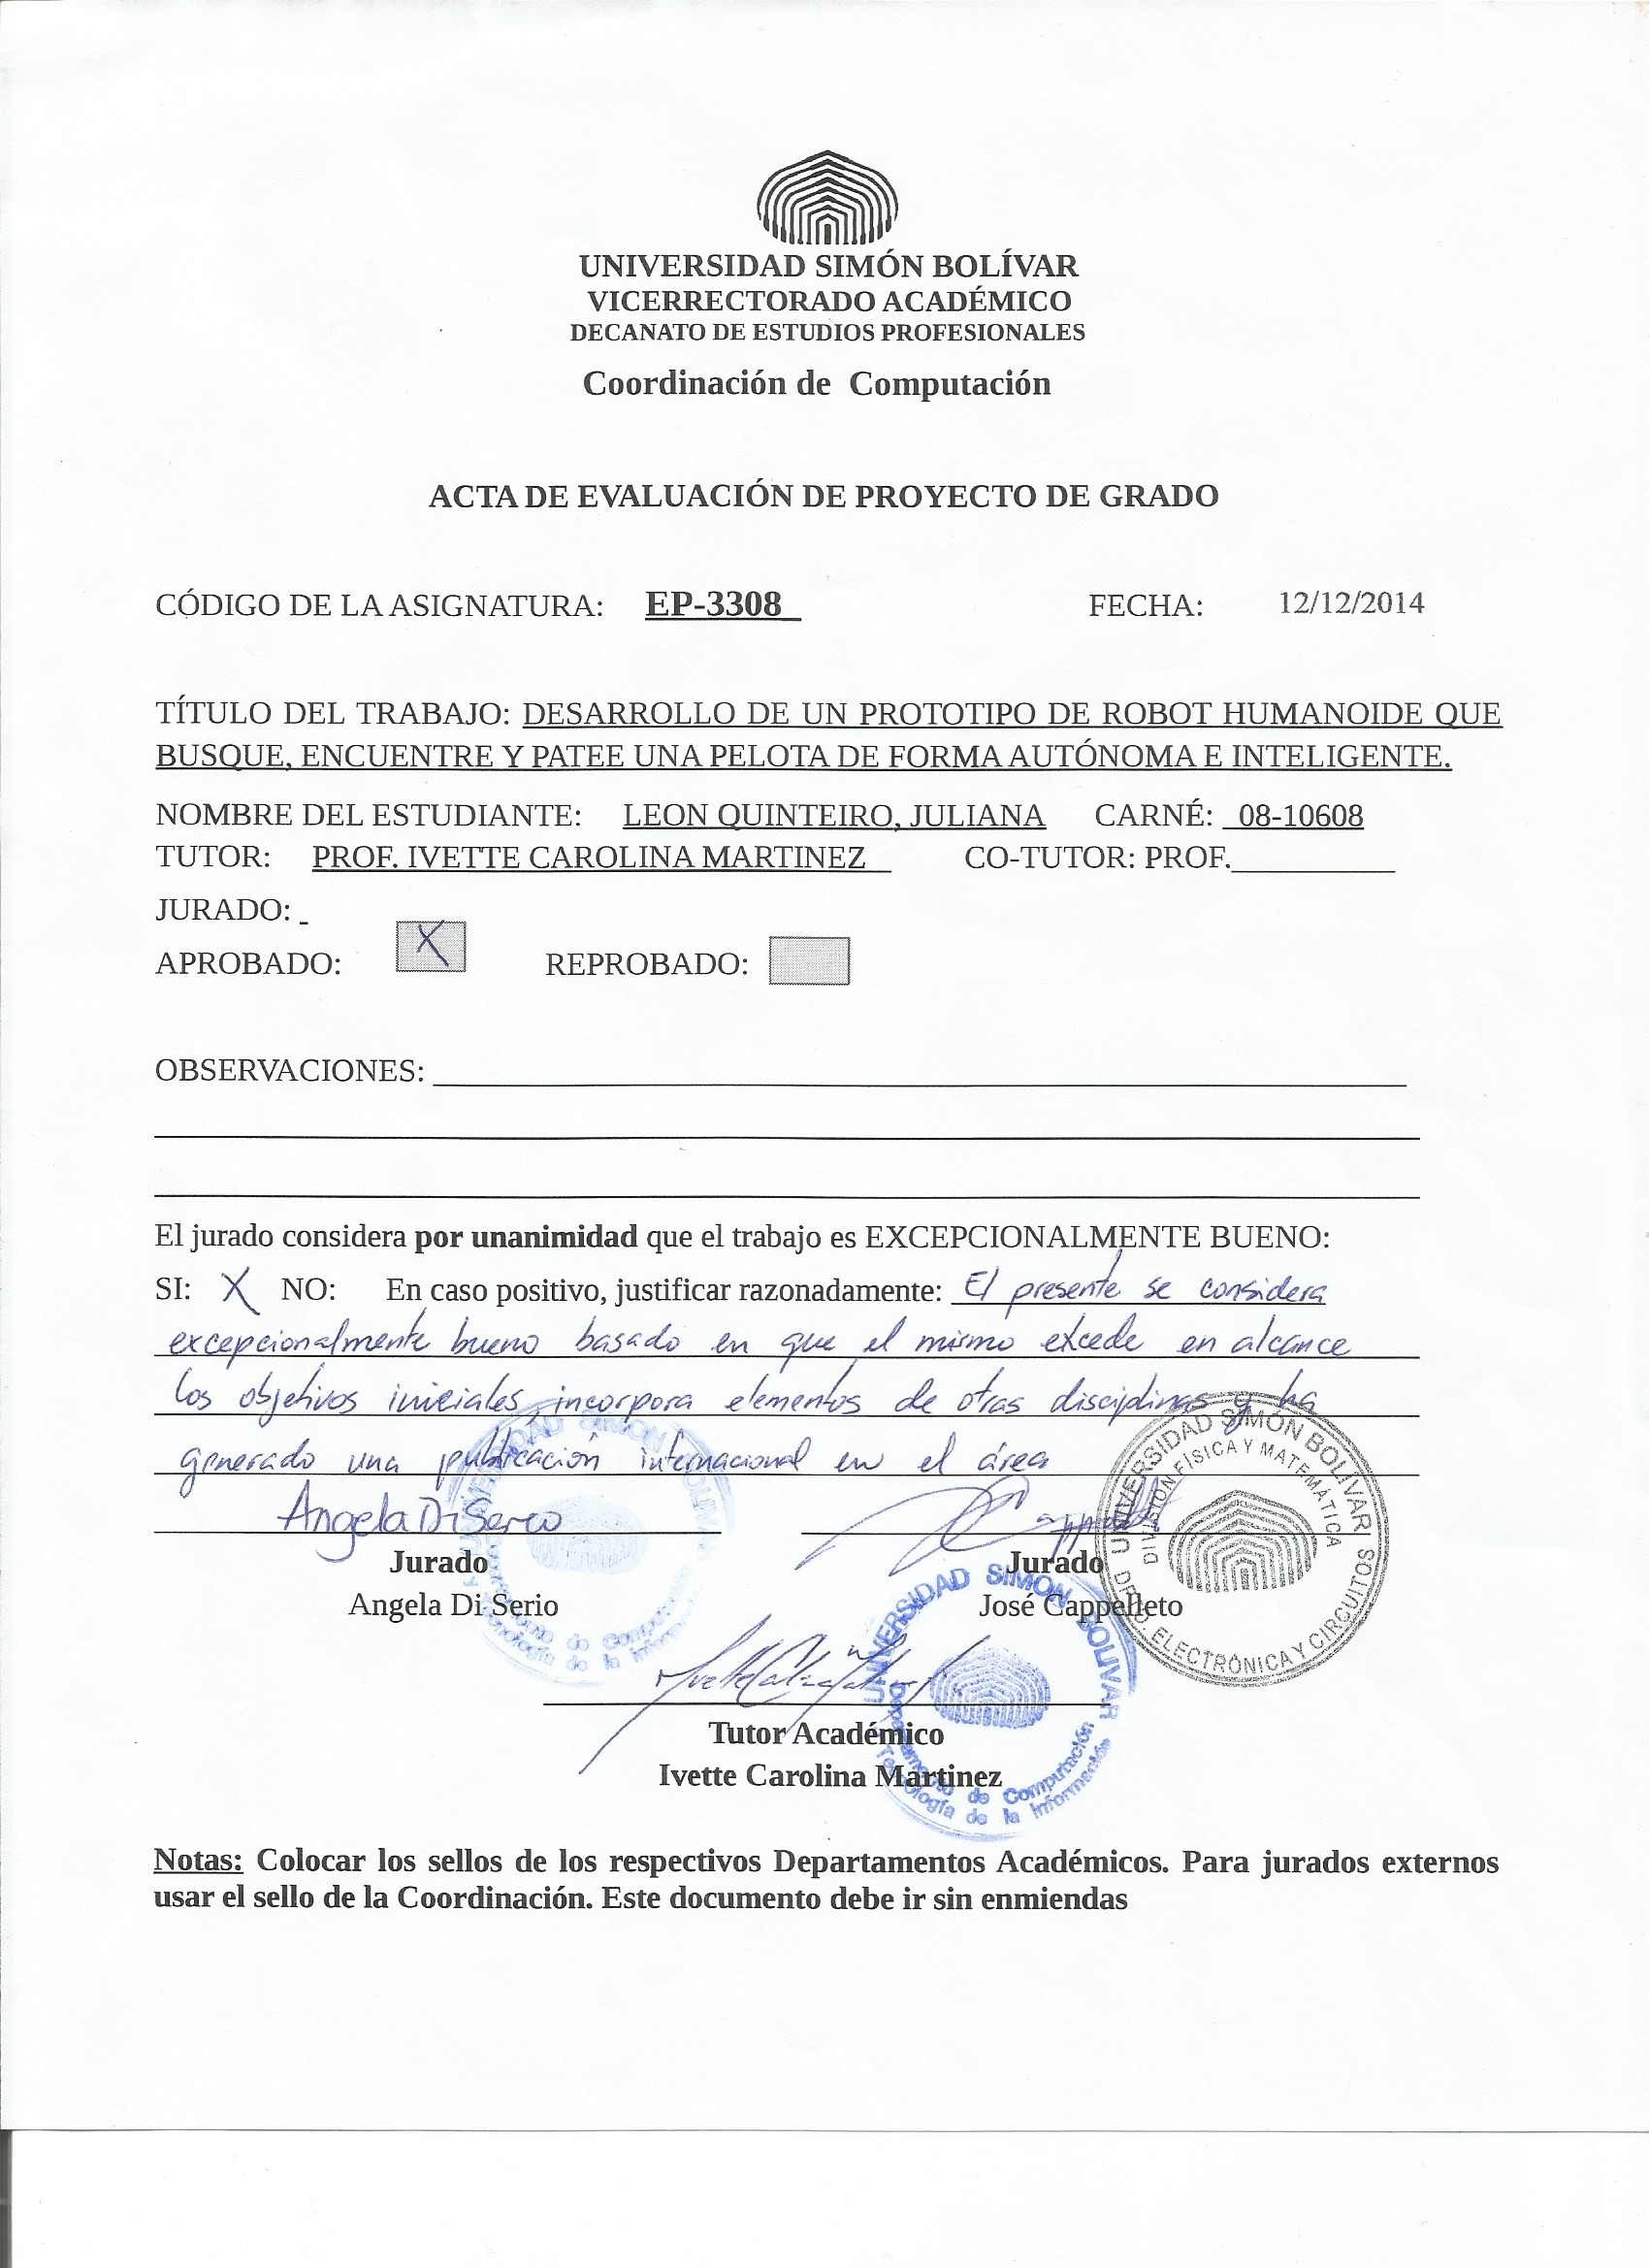
\includegraphics[width=\textwidth, height=\textheight]{figures/acta.jpg}

\setcounter{secnumdepth}{3}
\setcounter{tocdepth}{4}

% Define encabezado numeros romanos y como se separan los captiulos y las
% secciones
\addtolength{\headheight}{3pt}
\pagenumbering{roman}
\pagestyle{fancyplain}

\renewcommand{\chaptermark}[1]{\markboth{\chaptername\ \thechapter:\,\ #1}{}}
\renewcommand{\sectionmark}[1]{\markright{\thesection\,\ #1}}

\onehalfspacing

\lhead{}
\chead{}
\rhead{}
\renewcommand{\headrulewidth}{0.0pt}
\lfoot{}
\cfoot{\fancyplain{}{\thepage}}
\rfoot{}


% Pagina de resumen
\setcounter{page}{4}
\begin{center}
	{\bf Resumen} \pdfbookmark[0]{Resumen}{resumen} % Sets a PDF bookmark for the dedication
\end{center}	

%RoboCup \cite{robotcup} es una competencia de fútbol, iniciada en 1997, donde contribuyen las áreas de robótica, investigación e inteligencia artificial. Entre sus categorías se encuentra RoboCup Soccer \cite{robotcupsoccer}, la cual consiste en la participación de pequeños robots humanoides que se enfrentan a otro equipo para jugar fútbol.

En este proyecto se describe la construción de Junny, un robot humanoide autónomo e inteligente de $38 cm $ de alto, capaz de detectar la ubicación de una pelota y acercarse a ella para patearla con dirección al arco. Los objetivos de Junny están inspiradas en la liga RoboCup Soccer de la competencia RoboCup.

Junny ha sido ensamblado con las piezas del kit Bioloid Premium del fabricante Robotis. Del kit se ha excluido la tarjeta CM-510 para sustituirla por la tarjeta controladora Arbotix, la cual controla los 16 motores que permiten el movimiento de las extremidades del robot. Se ha incluido un mini computador Raspberry Pi, con su cámara, %\cite{raspberrycam},
de esta forma el robot ha adquirido la posibilidad detectar la posición de la pelota y el arco de forma autónoma. Se añadieron dos micro servomotores analógicos para ejecutar el movimiento de la c\'amara, estos son controlados por la tarjeta Arbotix. 

En la Raspberry Pi se ejecuta un solo programa encargado de detectar la posición de la pelota y decidir qué movimientos son necesarios para llegar a ella. La manera de elegir las acciones se ha realizado con aprendizaje por reforzamiento. Para filtrar y procesar la imagen se ha usado la segmentaci\'on por regiones para la detecci\'on de la pelota, con ayuda de las librerías OpenCv. % \cite{opencv}. 

La Arbotix, además de controlar los motores para ejecutar los movimientos deseados, se encarga de monitorizar la velocidad angular del robot, para ello usa el sensor Gyro de Robotics. Con esta información Junny puede deducir si se ha caído y levantarse. 
% Si detecta un desbalance de un cierto porcentaje 

Todos estos componentes deben ser coordinados para que se logre cumplir la tarea de seguir y patear la pelota. Por ello se hizo necesaria la comunicación entre la Arbotix y la Raspberry Pi. La herramienta 
empleada para ello ha sido el \gls{framework} \gls{ROS} (Ros Operating System). %\cite{ros}. 

Finalmente se obtuvieron los siguientes resultados, un robot aut\'onomo e inteligente que es capaz de reconocer la pelota, desplazarse hasta ella y patearla con direcci\'on al arco. Con la aplicaci\'on de aprendizaje por reforzamiento, se obtuvo un 100\% de aciertos, con una tasa de eficiencia de $0.72$ que es el n\'umero de acciones optimas entre las acciones realizadas. De los experimentos completos con la orientaci\'on al arco se obtuvo un 53 \% de orientaciones correctas con resultado de gol.

\textbf{Palabras claves}: Rob\'otica, Aprendizaje por reforzamiento, Humanoide, ROS, Arbotix.




% Pagina de dedicatoria (opcional)
\pagebreak

\setcounter{page}{5}

\vspace*{8cm} 
\pdfbookmark[0]{Dedicatoria}{dedicatoria} % Sets a PDF bookmark for the dedication
\begin{center} 
\large DEDICATORIA
\end{center}
\newpage


% Pagina de agradecimientos (opcional)
\setcounter{page}{6}

\chapter*{Agradecimientos
\markboth{Agradecimientos}{Agradecimientos}}
\pdfbookmark[0]{Agradecimientos}{agradecimientos}

\bigskip

AGRADECIMIENTOS



% Crea la tabla de contenidos
\tableofcontents

% Crea la lista de cuadros
\listoftables

% Crea la lista de figuras
\listoffigures

% Crea la lista de codigos fuentes
%\lstlistoflistings

\clearpage

% Define encabezado en numeros arabicos  
\pagenumbering{arabic}

\fancyhf{} % Redefine el encabezado 
\lhead{}
\chead{}
\rhead{\fancyplain{}{\thepage}}
\renewcommand{\headrulewidth}{0.0pt}
\lfoot{}
\cfoot{}
\rfoot{}

\doublespacing

% Incluye los archivos deseados - El contenido de su proyecto de grado/pasantia larga.
\chapter{Introducción}\label{intro}

\pdfbookmark[0]{Introducción}{introduccion} % Sets a PDF bookmark for the dedication

\label{sect:justificacion}
RobotCup \cite{robotcup} es una competencia de fútbol iniciada desde 1997 donde contribuyen las áreas de robótica, investigación e inteligencia artificial. Entre sus categorías se encuentra RobotCup Soccer \cite{robotcupsoccer}, la cual consiste en la participación de pequeños robots humanoides que se enfrentan a otro equipo para jugar fútbol. El objetivo de esta competencia es lograr que en el año 2050 el equipo campeón logre vencer al ganador del año en la copa mundial de la FIFA (International Federation of Association Football). Las destrezas de robots con forma de humanos (como son caminar, percibir el mundo y tomar alguna acción sobre él) suelen ser más complejas de lo que se puede pensar. Una de las más avanzadas muestras en el área es el robot ASIMO \cite{asimo}, creado por la compañía Honda, cuyos últimos avances incluyen la predicción de trayectoria de objetos para poder esquivarlos.

En este proyecto se presenta un robot humanoide (Debupa) de tamaño pequeño (38 cm de altura) cuyos objetivos estan basados en las reglas de la competencia RobotCup. En artículos de este mismo enfoque se puede encontrar el trabajo de Sven Behnke cuyo título es “See, walk, and kick: Humanoid robots start to play soccer” donde se describe la construcción del equipo de robots que participaron en la RobotCupSoccer en el a\~no 2006. El artículo cubre el diseño mecánico y electrónico, además el software utilizado para la percepción, control de comportamiento, comunicación y simulación de los robots. \cite{paper}.

Existen equipos que han participado durante varios años consecutivos en la competencia Robocup, logrando mejoras en sus diseños y técnicas; tal es el caso del equipo MRL que ha participado en los años 2011, 2012, 2013 y 2014 en la categoría “Humanoid League”, han iniciado con el hardware del robot DARwIn-OP y con el tiempo han modificado los componentes electrónicos para agregar eficiencia y estabilidad. Para el balance han utilizado un giróscopio y sensores de aceleración, y para la visión una cámara conectada por usb al CPU principal \cite{paper1}.

En el desarrollo de habilidades más específicas con respecto a la competencia RobotCup Soccer, en el artículo de investigación de Seung-Joon Yi, Stephen McGill y Daniel D. Lee  \cite{paper2}, se refieren a dos posibles estrategias para el pateo de la pelota donde los factores fundamentales para un buen desempeño es la fuerza y la rapidez con que se patea, los investigadores ponen en pr\'actica dos estrategias de pateo en distintas circunstancias del juego basado en la cinemática y dinámica de equilibrar el cuerpo al momento de realizar el pateo.

El objetivo general de este proyecto se basa en construir un prototipo de robot humanoide que sea capaz de detectar la cercanía
de una pelota, acercarse a ella y patearla, reincorporandose a la posicion de pie en caso de perder el equilibrio y caer
mientras camina. Para cumplir con este objetivo se ha desglosado un conjunto de objetivos específicos que se describen 
a continuación: 

\begin{enumerate}
\item  Diseño y construcción de un humanoide con piezas del kit de robótica Bioloid Premium, sustituyendo su tarjeta controladora
CM-530 por la tarjeta de software libre ArbotiX para controlar los motores Dynamixel y otros sensores.
\begin{enumerate}
\item Instalación y configuración de la tarjeta ArbotiX.
\item Instalación y configuración de la tarjeta Raspberry Pi.
\item Instalación y configuración de la cámara Raspberry Pi.
\item Instalación de servomotores  para el movimiento de la cámara
\item Instalación del giroscopio Gyro.
 
\end{enumerate}
\end{enumerate}

\begin{enumerate}
\item Detección de la pelota
\begin{enumerate}
\item  Captura de imagen con la cámara Raspberry Pi a través de la librería raspicam cv.
\item Procesamiento de la imagen para extraer información de la posición de la pelota con las librerías de OpenCV.
\end{enumerate}

\end{enumerate}

\begin{enumerate}
\item Búsqueda de la pelota y pateo de la misma. 
\begin{enumerate}
\item Creación de las poses necesarias para caminar, girar, levantarse y patear usando el software pypose.
\item Programación de transiciones de movimientos.
\item Control de servomotores para el movimiento de la cámara.
\item Establecer mecanismo de comunicación entre la tarjetas ArbotiX y Raspberry Pi.  
\item Programación de algoritmo de planificación de acciones que lleve al humanoide a acercarse a la pelota.
\item Detección de movimientos angulares bruscos que sugieran una caída, a través de la lectura del giroscopio
\item Identificación del momento en que la pelota se encuentre en una zona adecuada para patear.
\end{enumerate}
\end{enumerate}

En el capítulo (\ref{chapter:Tecnologias_utilizadas}) se describen los componentes de hardware usados para construir el humanoide; luego en la sección \ref{sec:Estru}
se explica cómo se unieron esas piezas. Con respecto a la parte de programación, en la secci\'on \ref{sec:Movimientos} se describe c\'omo se logró constituir los movimientos necesarios para que el humanoide cumpla sus objetivos, mientras que en la secci\'on \ref{sec:resultados} se muestran los resultados experimentales. Las herramientas y técnicas  que  permitieron lograr  la detección de la pelota se detallan en la secci\'on \ref{sec:vision_del_robot}. También se describe la discretización del ambiente para reducir el n\'umero de estados. La comunicación de las tarjetas Arbotix y Raspberry Pi para que puedan trabajar en conjunto se explica en la secci\'on \ref{sec:integracion_de_componentes}  y consideraciones especiales en la secci\'on \ref{sec:consideraciones}.


% Marco Teorico.
\chapter{Marco teórico} \label{chap:marco_teorico}
\vspace{5 mm}
En este capítulo se presentan los conceptos que conforman la base teórica para comprender este trabajo. Primero se brinda una descripción de los términos relativos a la robótica y las partes principales de un robot. Posteriormente se describen algunos conceptos que tienen que ver con la robótica inteligente, como los paradigmas, la inteligencia y la visión artificial para la detección de objetos. 
\section{Robótica} \label{sect:robotica}
 
Para definir un lenguaje formal se requiere describir:
\begin{itemize}
\item{\textbf{Robot:} Es un agente artificial, activo, cuyo entorno no es el mundo físico. El término activo descarta de esta definición a las piedras, el término artificial descarta a los animales, y el término físico descarta a los agentes de software puros o softbots, cuyo entorno lo constituyen los sistemas de archivos, bases de datos y redes de cómputo. \cite{peterNorvig}}

\item{\textbf{Robótica:} Es la rama de la tecnología que se encarga del diseño, construcción, operación y aplicación de los robots. \cite{oxfordRobotics}}

\item{\textbf{Sensores:}  Son los encargados de percibir el ambiente que rodea al robot. Según Murphy R.R son dispositivos que miden algún atributo del mundo. Un sensor recibe energía del entorno (sonido, luz, presión, temperatura, etc) y transmite una señal a una pantalla o computador ya sea de forma análoga o digital. \cite{AiRobotics}}

\item{\textbf{Actuador:}  Es aquella parte del robot que convierte comandos de software en movimientos físicos.  \cite{peterNorvig}}

\item{\textbf{Servomotor:}  Es un motor eléctrico, considerado como actuador, que permite ser controlado tanto en velocidad como en posición. }

\item{\textbf{Giróscopio:} Es un sensor utilizado para medir y mantener la orientación, se mide a través del momento angular. \cite{gyro1}}
\end{itemize}

%****************************************************************************************/
\section{Robótica Inteligente (Agentes Inteligentes)} \label{sect:AgentesInteligentes}
\subsection{Paradigmas de robótica}
En la robótica inteligente, según Robin Murphy, existen tres paradigmas en los cuales se clasifica el diseño de un robot inteligente, estos paradigmas pueden ser descritos de dos maneras: la relación entre las primitivas básicas de la robótica, percibir, planificar, actuar o de la forma en que los datos son percibidos y distribuidos en el sistema.

Percibir se refiere al procesamiento útil de la información de los sensores del robot. Planificar, cuando con información útil, se crea un conocimiento del mundo y se generan ciertas tareas que el robot podría realizar. Por último actuar consiste en realizar la acción correspondiente con los actuadores del robot para modificar el entorno. 

\subsubsection{ Paradigma Jerárquico}

Este paradigma es secuencial y ordenado. Primero el robot percibe el mundo y construye un mapa global. En base al mapa ya percibido y con “los ojos cerrados”, el robot planifica todas tareas necesarias para lograr la meta. Luego ejecuta la secuencia de actividades según la planificación realizada. Una vez culminada la secuencia se repite el ciclo percibiendo el mundo, planificando y actuando. \cite{AiRobotics}

\subsubsection{Paradigma Reactivo}
El paradigma reactivo omite por completo el componente de la planificación y solo se basa en percibir y actuar. El robot puede mantener un conjunto de pares percibir-actuar, estos son llamados comportamientos y se ejecutan como procesos concurrentes. Un comportamiento toma datos de la percepción del mundo y los procesa para tomar la mejor acción independientemente de los otros procesos. \cite{AiRobotics}

\section{Inteligencia Artificial} \label{sect:Inteligencia_Artificial}
La inteligencia artificial es un término relacionado con la computación y la robótica que ha tenido varias definiciones, ocho de ellas, las cuales nacieron a finales del siglo XX, se encuentran organizadas en \cite{peterNorvig} bajo cuatro categorías: pensar y actuar de forma humana, pensar y actuar de forma racional. Con ello se puede entender que la inteligencia artificial tiene que ver con lograr que un robot resuelve problemas de manera inteligente, es decir, de manera que parezca que el razonamiento y comportamiento humano las ha resuelto.  

\subsection{ Aprendizaje de Máquinas}
El aprendizaje de máquinas es un área de la inteligencia artificial que está relacionada con la pregunta de cómo construir programas de computadora que automáticamente mejoren con la experiencia. Se dice que un programa aprende de la experiencia E con respecto a una tarea T y desempeño P si el desempeño en la tarea T, medido por P, mejora con con la experiencia E \cite{Mitchell}.
\subsection{Aprendizaje por reforzamiento}
El aprendizaje por reforzamiento es un tipo de aprendizaje de máquinas que se basa en un sistema de recompensas y penalizaciones. Las recompensas se pueden dar en cada estado o una sola vez al llegar al estado final.

El objetivo del agente es aprender de las recompensas para escoger la secuencia de acciones que produzca la mayor recompensa acumulada. \cite{Mitchell}

El agente existe en un entorno descrito por algunos estados S. Puede ejecutar un conjunto de acciones A. Cada vez que ejecuta una acción $a_t$ en algún estado $s_t$ el agente recibe una recompensa $r_t$. El objetivo es aprender una política $\pi$ : S $\to$ A que maximice la suma esperada de esas recompensas con descuento exponencial de las recompensas futuras. \cite{Mitchell} El resultado de tomar las acciones puede ser determinista o no, en el caso de este proyecto no es determinista, es decir, existen porcentajes de probabilidad de pasar a un estado u otro al tomar una acción en un estado en particular.  
\subsection{ Q- learning}

Es un método de aprendizaje por reforzamiento que, dado un estado, compara las utilidades esperadas de las posibles acciones a tomar sin necesidad de saber el estado resultante, por tanto no se necesita tener un modelo del entorno \cite{peterNorvig}.

La forma de aprender la política $\pi$ : S $\to$ A es de forma indirecta, a través de la función $Q(s,a)$. La función esta definida como el valor de la máxima recompensa acumulada con descuento que puede ser alcanzada desde el estado $s$ y aplicando $a$ como la primera acción. Es decir, el valor de Q es la recompensa recibida inmediatamente 


\section{Visión Artificial} \label{sect:Vision_Artificial}

Una manera de obtener información del ambiente es con la visión artificial. Esta consiste en usar un dispositivo (cámara) que
capta el espectro electromagnético y produce una imagen. La representación de la imagen se almacena como una matriz de píxeles,
cada píxel es un elemento que guarda información de una región en el espacio captado. Si se usa una cámara de luz, la información
de cada píxel será el color. \cite{AiRobotics}  

Por lo general luego de obtener una imagen se requiere extraer información de ella, por lo cual se han desarrollado diferentes algoritmos y t\'ecnicas que ayudan en esta tarea. En la sección \ref{sec:Segmentacion} se describe la t\'ecnica de segmentaci\'on por regiones, que es la utilizada en esta proyecto. 

Por otro lado, existen varios algoritmos que se dedican a la transformación de las imágenes para reducir
ruidos, compensar problemas de iluminación, extraer formas, identificar objetos, entre otros. En esta sección se describen dos de las técnicas de transformación para reducir el ruido basadas en la dilatación y erosión de la imagen (secci\'on \ref{sec:Transfor}). 
 
\subsection{Segmentaci\'on por regiones}\label{sec:Segmentacion}

La pr\'actica m\'as general en visi\'on de computadoras aplicado a rob\'otica es la identificaci\'on de regiones por un color particular, este proceso se llama segmentaci\'on por regiones. El algoritmo b\'asico consiste en identificar todos los p\'ixeles en una imagen que forman parte de una regi\'on y luego navegar al centro de la regi\'on. El primer paso es identificar todos los p\'ixeles en la imagen que compartan un rango de valores con el color particular y agruparlos, aquellos p\'ixeles que no compartan el color son descartados \cite{BookOpenCv}. 

\subsection{Filtros}
El filtrado de imágenes es una técnica para la transformación de imágenes, que consiste en destacar  sus características más relevantes en base a un propósito en particular. 

Generalmente en la tarea de extracción de información de una imagen se utilizan filtros para descartar zonas o características que no son importantes para el patrón deseado y para determinar el área deseada ya sea por patrones de forma o color.

En la investigación, los algoritmos de filtrado aplicados a las imágenes fueron: Clausura Morfológica y Apertura Morfológica, filtros que aplican las técnicas de erosión y dilatación a las imágenes.

\subsection{Transformaciones Morfológicas}\label{sec:Transfor}
Las transformaciones morfológicas básicas son llamadas dilatación y erosión, se utilizan en 
amplia variedad de contextos como la eliminación del ruido, aislamiento de elementos individuales y elementos de unión dispares
en una imagen.\cite{BookOpenCv}

\subsubsection{Dilatación}
La dilatación es una convulsión (algo que se le aplica a toda la imagen) entre alguna imagen (o región de una imagen), que llamaremos A y un núcleo que llamaremos B, el núcleo, que puede ser de cualquier forma o tamaño, tiene un solo punto de anclaje definido. Para mayor claridad el n\'ucleo es esencialmente una matriz de tamaño fijo  de coeficientes numéricos junto con un punto de anclaje en dicha matriz, que normalmente se encuentra en el centro . Muy  a menudo, el núcleo es un pequeño cuadrado o disco sólido. El núcleo puede ser pensado como una plantilla  o m\'ascara, y su efecto para la dilatación tal como un operador de máximo local sobre la imagen, se calcula el m\'aximo valor de los píxeles común a B y reemplazamos el píxel de la imagen en el punto de anclaje con ese valor máximo. Esto causa regiones brillantes dentro de una imagen y la hacen crecer. Este crecimiento es el origen del término `` operador de dilatación" \cite{BookOpenCv}. 

\begin{figure}[hbtp]

\centering
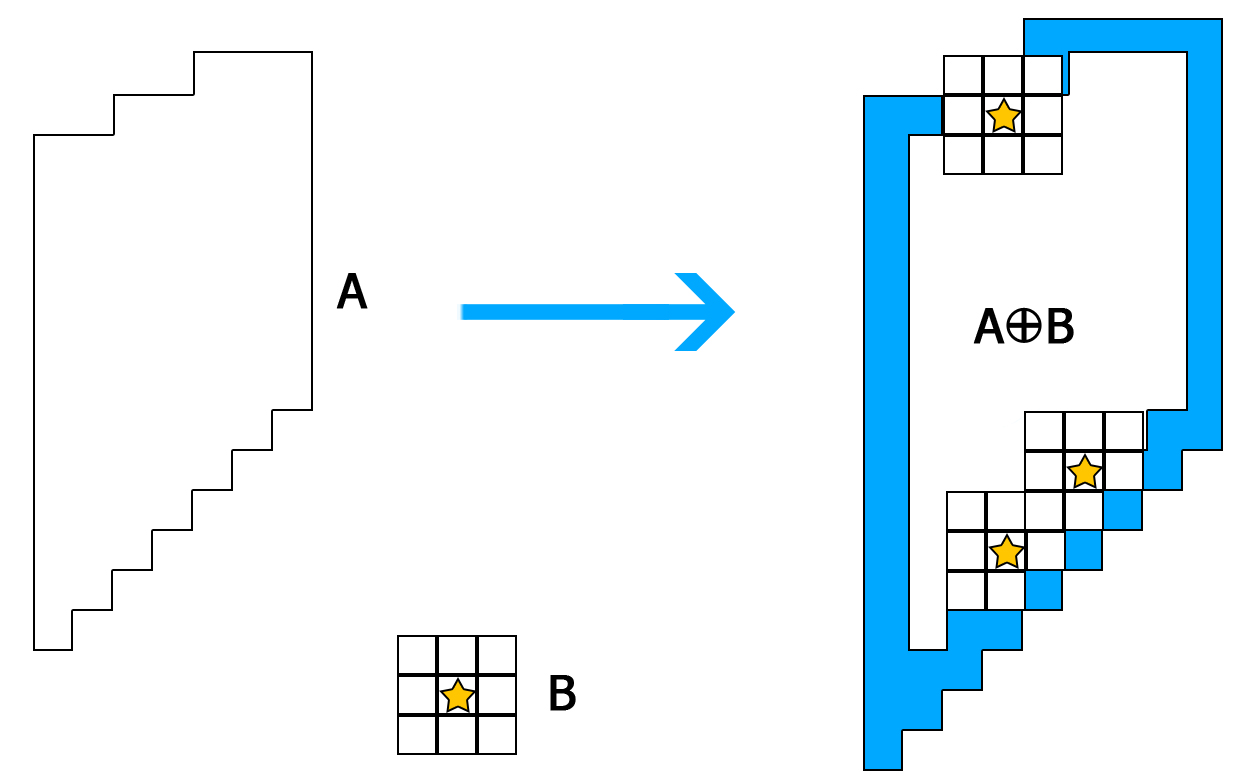
\includegraphics[scale=0.2]{imagenes/erosion-model.jpg}
\caption{Dilatación}
\end{figure}

\subsubsection{Erosión}
La erosión es la operación inversa a la dilatación. Esta acción del operador es equivalente a el cálculo de un mínimo local sobre el área del núcleo. La erosión genera una nueva imagen a partir de la original, utilizando el siguiente algoritmo: como el núcleo B es analizado sobre la imagen, se calcula el mínimo valor del píxel superpuesto por B y se reemplaza el píxel de la imagen con un punto de anclaje de valor mínimo \cite{BookOpenCv}. 
V\'ease en la figura \ref{fig:erosion}

\begin{figure}[hbtp]
\centering
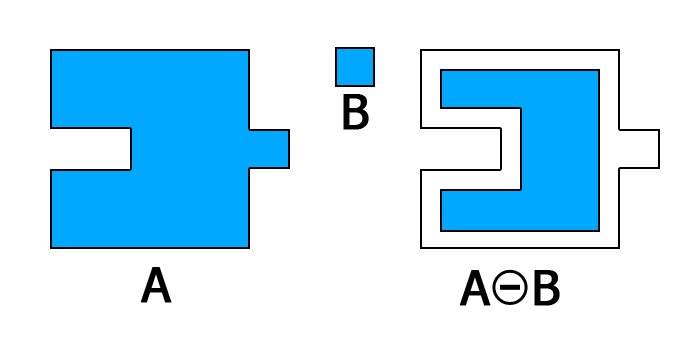
\includegraphics[scale=0.5]{imagenes/erosion.jpg}
\caption{Erosión}
\label{fig:erosion}
\end{figure}





\chapter{Tecnologías utilizadas}\label{chapter:presentacion_del_problema}

 PODRIA IR ACA LA PRESENTACION DEL PROBLEMA
 
 OBJETIVOS
 
\section{ Herramientas de software}
En esta sección se describen las herramientas de software utilizadas para la programación del proyecto.
\begin{itemize}
\item Pypose: Software especializado en el control de los servomotores Dynamixel Ax-12. Una de las más importantes características es que, luego de haber fijado a mano las posiciones de los motores, permite la lectura simultánea de esas posiciones para captar la pose del robot. Con esta herramienta es posible formar una secuencia de poses que generen un movimiento, por ejemplo, caminar. \cite{pypose}

\item ROS: ROS (Robot Operating System) es un framework que proporciona bibliotecas y herramientas para ayudar a los desarrolladores de software a crear aplicaciones robóticas. Proporciona abstracción de hardware, controladores de dispositivos, bibliotecas, visualizadores, paso de mensajes, gestión de paquetes y más. ROS se encuentra bajo licencia de código abierto, la licencia BSD.

\item OpenCv (Open Source Computer Vision Library): Es una librería de visión de computadoras y aprendizaje de maquinas de código abierto. Ha sido diseñada para acelerar el uso de la percepción de maquinas y para proveer una estructura común en las aplicaciones de visión de computadoras. Registrada bajo la licencia BSD, de código abierto. \cite{opencv}

\item IDE Arduino: Es un entorno de desarrollo para escribir y cargar código en la tarjeta Arduino. Otras tarjetas con microcontroladores AVR también son compatibles, como la Arbotix. El lenguaje de programación del IDE de Arduino es una implementación de Wiring el cual esta basado en Processing.  \cite{arduino}

\end{itemize}


\section{Componentes de hardware}
En esta sección se describen los principales componentes utilizados para armar la estructura del robot.
\begin{itemize}
\item Bioloid Premium kit: Es un kit de robótica con piezas modulares que permite armar diferentes tipos de robot pero principalmente humanoides. El fabricante, ROBOTIS, incluye un manual con varios modelos de robots con instrucciones de ensamblaje. Provee una tarjeta controladora, CM-530, a la que se conectan los motores Dynamixel y algunos sensores que se programan a través de la interfaz de ‘RoboPlus’.

\end{itemize}

\begin{figure}[hbtp]

\centering
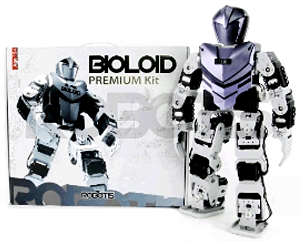
\includegraphics[scale=0.5]{imagenes/product_bioloid17.png}
\caption{Bioloid Kit}
\end{figure}

\begin{itemize}

\item Motores Dynamixel Ax-12+: Son actuadores inteligentes y modulares que incorporan un reductor de engranajes, un motor DC de presión y un circuito de control con funcionalidad de red, todo en un solo paquete. (R. INC, Dynamixel AX-12, 2006.)
\end{itemize}

\begin{figure}[hbtp]

\centering
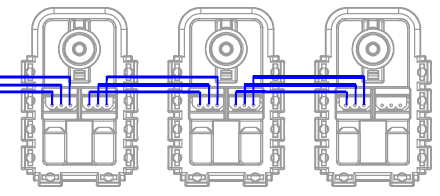
\includegraphics[scale=0.5]{imagenes/AX-12_serie.png}
\caption{Motores Dynamixel conectados en serie}
\end{figure}

\begin{itemize}
\item Gyro: Es un giroscopio de la marca Robotis que mide la velocidad angular, diseñado para mantener el balance del robot y ser usado para otras aplicaciones de movimiento. 

\end{itemize}

\begin{figure}[hbtp]
\centering
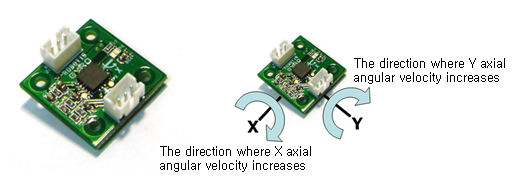
\includegraphics[scale=0.5]{imagenes/gyro.png}
\caption{Sensor Gyro }
\end{figure}

\begin{itemize}
\item Arbotix: El controlador ArbotiX es una solución de control avanzado para manejar servos Dynamixel AX/MX/RX/EX y robots basados en Bioloid. Incorpora un potente microcontrolador AVR, radio inalámbrica XBEE, conductores de motor dual, y cabeceras de estilo servo de 3 pines para E/S digital y analógica.\cite{arbotix}

\end{itemize}


\begin{itemize}
\item FTDI (Future Technology Devices International) : Es una tarjeta controladora que ofrece el servicio de conversión de datos de USB a UART. Permite la comunicación entre diferentes dispositivos. 


\end{itemize}
\begin{figure}[hbtp]

\centering
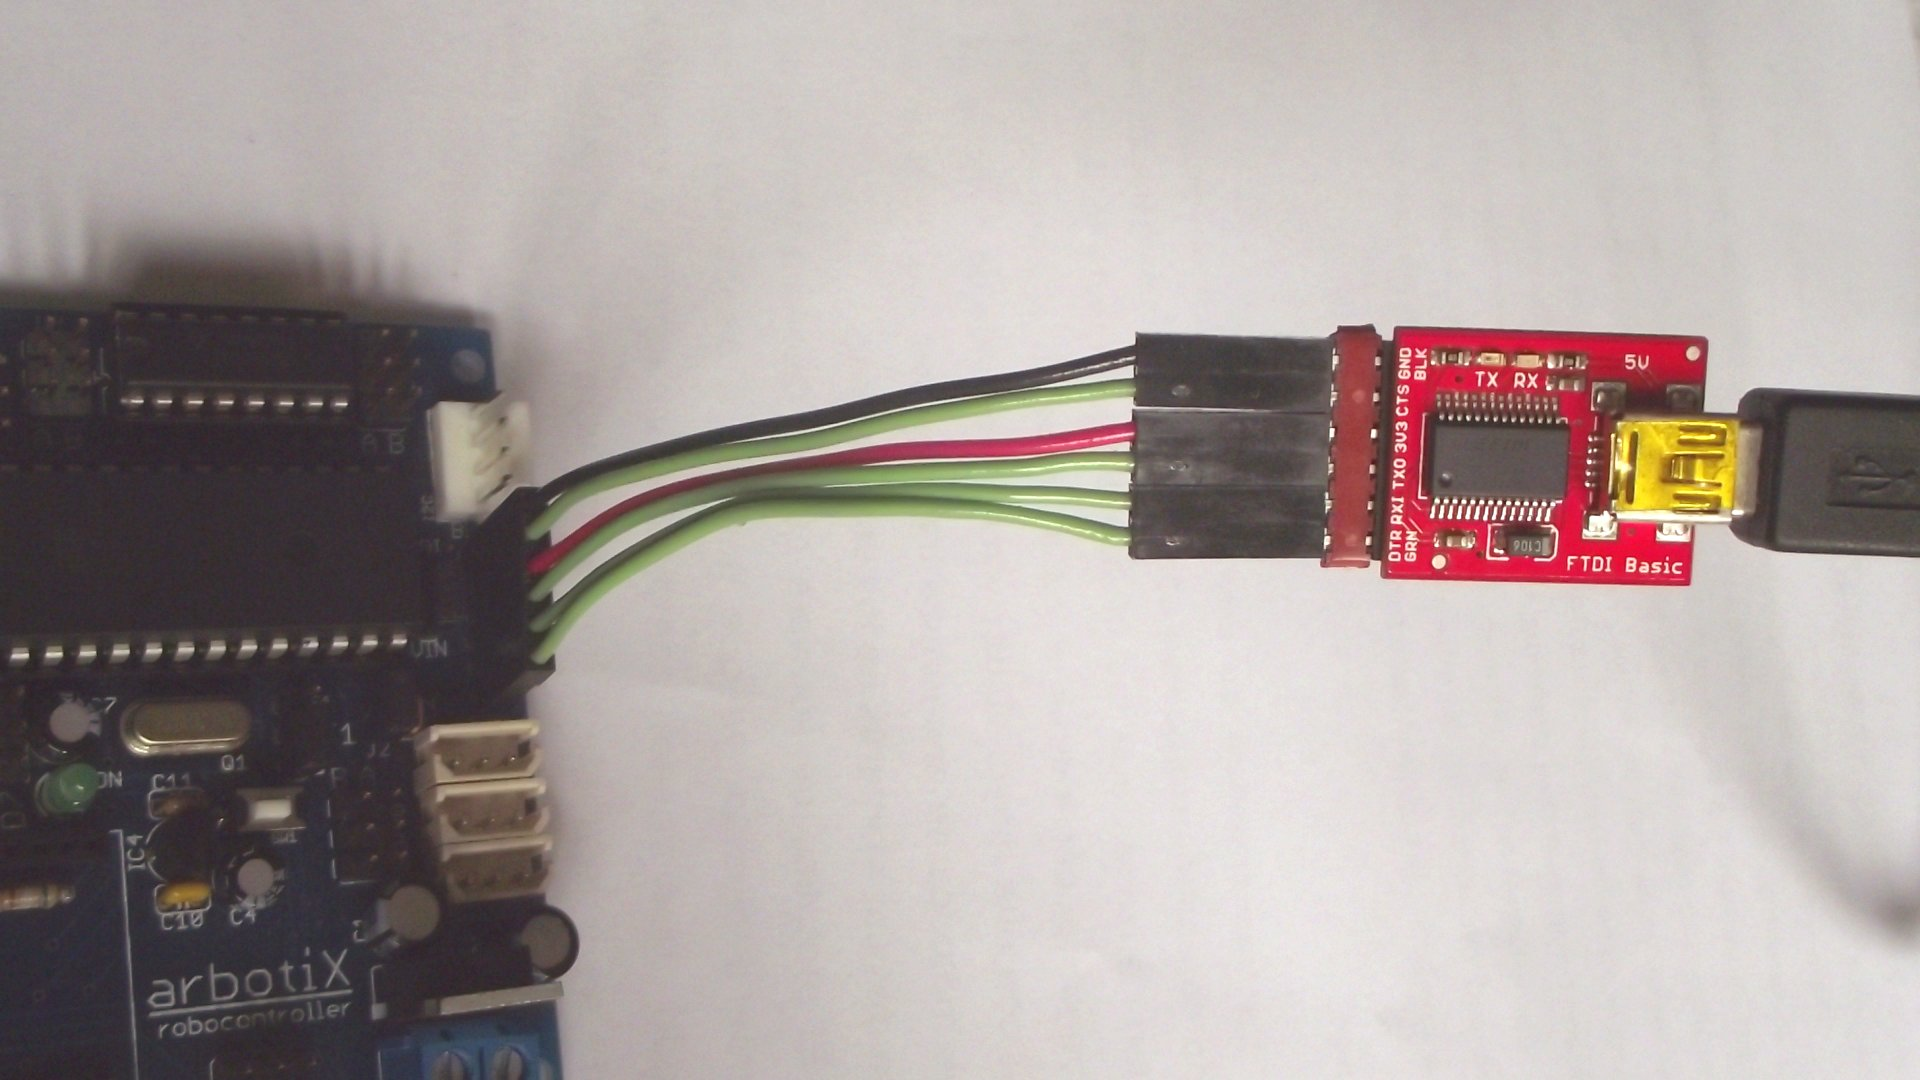
\includegraphics[scale=0.09]{imagenes/DSCF1162.jpg}
\caption{Chip FTDI conectado a la tarjeta Arbotix }
\end{figure}



\begin{itemize}
\item Extensor de puertos bioloid : Permite aumentar el número de cadenas de servos conectados a la tarjeta. 

%https://www.bananarobotics.com/shop/Dynamixel-AX-MX-6-Port-Extension-Hub

\end{itemize}


\begin{figure}[hbtp]

\centering
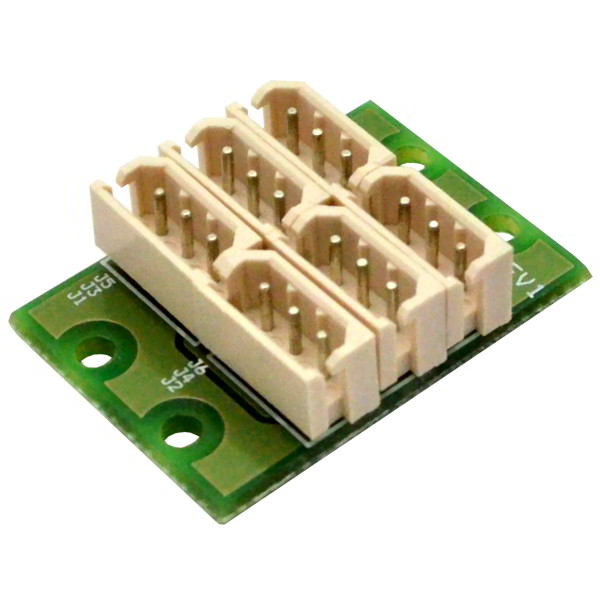
\includegraphics[scale=0.3]{imagenes/Dynamixel-AX-MX-6-Port-Extension-Hub-600x600.jpg}
\caption{Extensor de puertos bioloid  }
\end{figure}


\begin{itemize}
\item Servo motor analogico micro TG9 e: Es un pequeño servomotor cuyo torque alcanza 1.50 kg-cm y una velocidad de 60º por segundo. Permite ser controlado en posición en un rango de 180º. 

%http://www.hobbyking.com/hobbyking/store/__9549__Turnigy_TG9e_9g_1_5kg_0_10sec_Eco_Micro_Servo.html

\end{itemize}


\begin{figure}[hbtp]

\centering
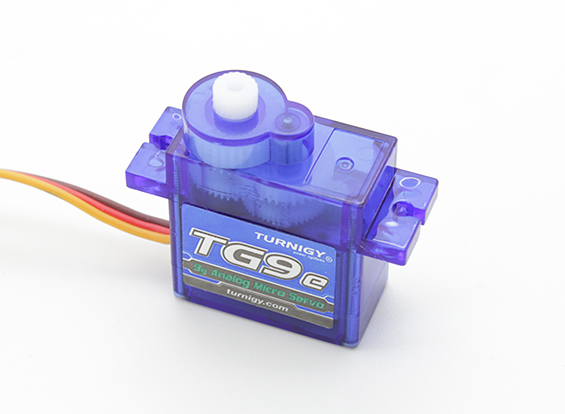
\includegraphics[scale=0.3]{imagenes/turnigy.jpg}
\caption{Servo motor analogico}
\end{figure}

\begin{itemize}
\item Raspberry Pi: La Raspberry Pi es un ordenador del tamaño de una tarjeta de crédito a la que se puede conectar un televisor y un teclado. Se trata de un pequeño ordenador capaz de ser utilizado en proyectos de electrónica, y para muchas de las tareas que una PC de escritorio hace, como hojas de cálculo, procesadores de texto y juegos. http://www.raspberrypi.org/ 



%imagen tomada de: %http://rayhightower.com/blog/2012/12/03/ruby-on-raspberry-pi/

\end{itemize}
\begin{figure}[hbtp]

\centering
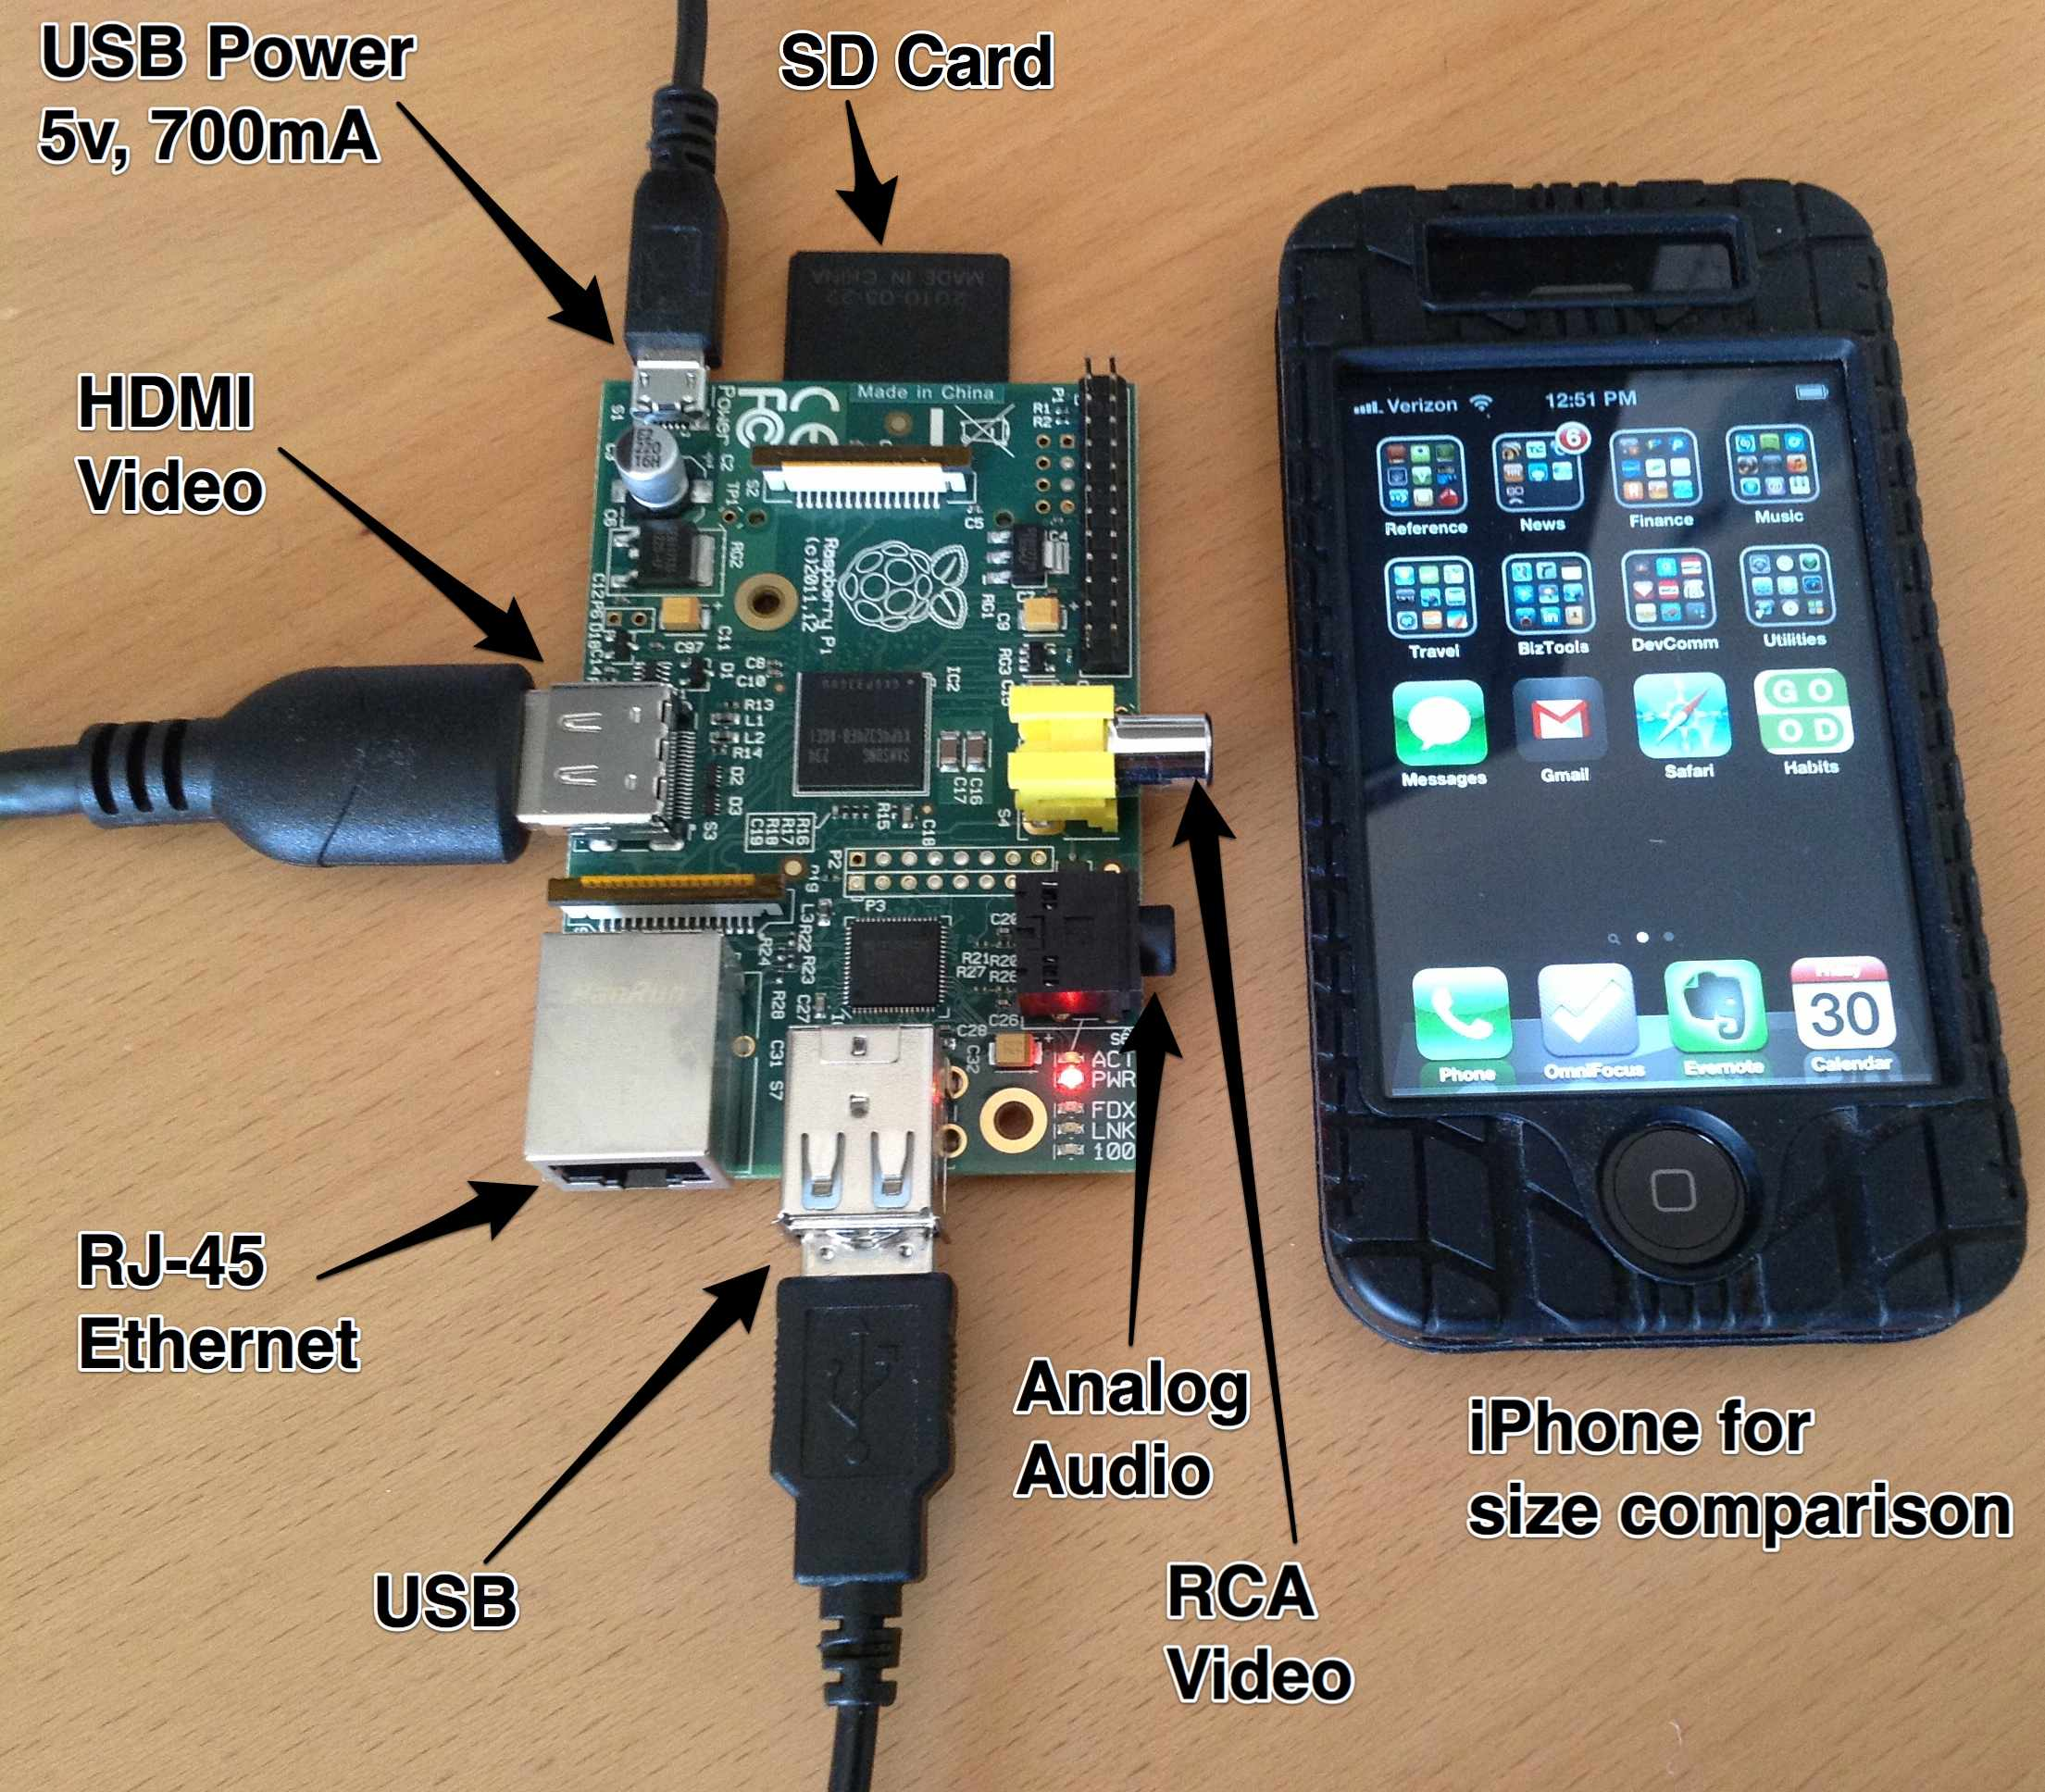
\includegraphics[scale=0.1]{imagenes/raspberry_pi_iphone.jpg}
\caption{Tarjeta Raspberry Pi con descripción de los puertos}
\end{figure}

\begin{itemize}
\item Camara Raspberry Pi: Es un sensor encargado de captar imagenes y grabar videos de alta definicion. Se conecta a la Raspberry Pi con un cable de cinta plana de 15 cm en el puerto CSI. Tiene 5 megapíxeles de foco fijo que soporta los modos de vídeo de 1080x30, 720x60 y VGA90. Puede ser manejada con las librerías MMAL, V4L u otras librerías de terceros como la de Python. %(http://www.raspberrypi.org/products/camera-module/)

\end{itemize}

\begin{figure}[hbtp]

\centering
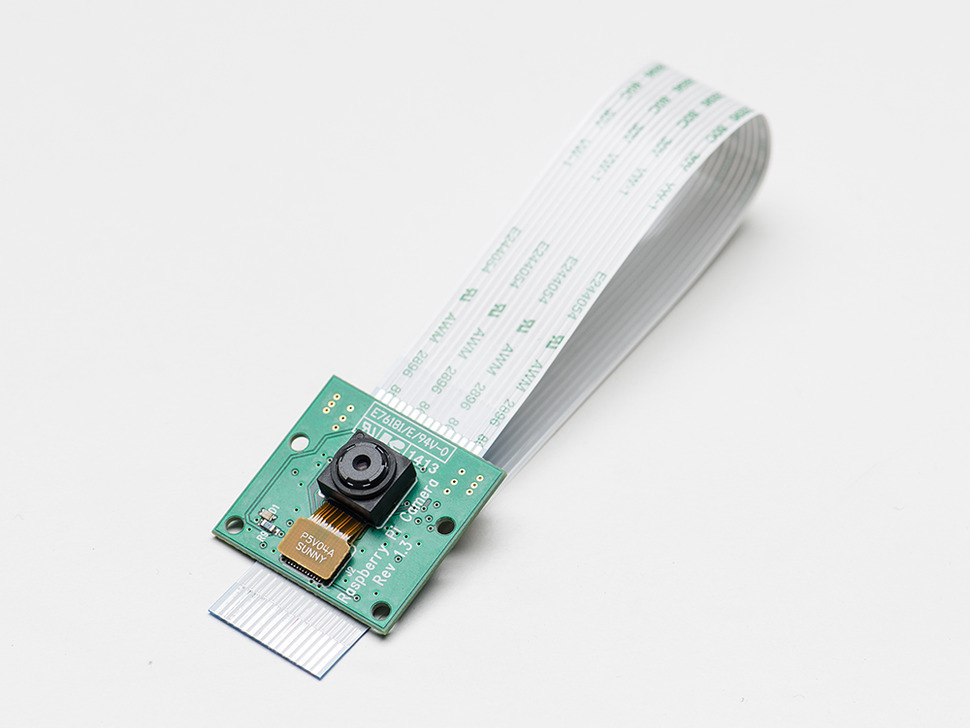
\includegraphics[scale=0.7]{imagenes/1367-01.jpg}
\caption{Camara Raspberry Pi}
\end{figure}


\begin{itemize}
\item Batería de polímero de litio (Lipo): Es la fuente de poder usada para que los motores y componentes electronicos funcionen. La batería usada es de 11.1 voltios y 1 amperio. 
\end{itemize}


\begin{figure}[hbtp]

\centering
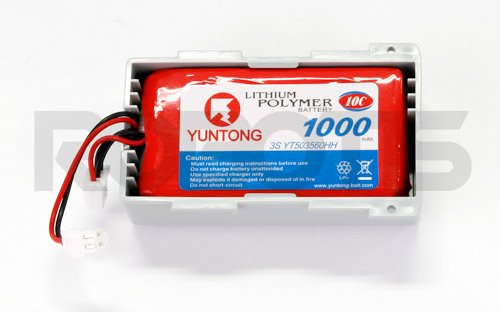
\includegraphics[scale=0.7]{imagenes/R-LIPOBAT.jpg}
\caption{Lipo}
\end{figure}

\begin{itemize}
\item Circuito con regulador de 5v: Es un circuito diseñado y construido para este proyecto cuya finalidad es regular la entrada de la corriente. Por una de las salidas se expulsa 5v y por la otra se mantiene el mismo voltaje de entrada. 

\end{itemize}




\chapter{Definición de lenguaje}\label{chapter:def_lenguaje}

\textbf{Amorfinator} es un lenguaje desarrollado con la finalidad de facilitar la 
generación de instancias aleatorias de estructuras de datos. Por ende, está 
diseñado para proporcionar a sus usuarios una sintaxis intuitiva que permita 
especificar la estructura final deseada, así como las funciones para verificar 
u obtener valores y también las estructuras auxiliares que sirven como 
herramientas para obtener los resultados finales.

La sintaxis fue diseñada para aceptar palabras reservadas escritas tanto en
ingles como en español, incluso en ambos idiomas al mismo tiempo.

%----------------------------- Estructura general -----------------------------%
\section{Estructura general}
La estructura general se basa en la idea de centrar toda la importancia en una 
única estructura de salida, que contendrá la definición del objeto deseado a 
generar. Para facilitar esto, se decidió diseñar una estructuración por bloques 
que separen la salida final de otras instancias auxiliares y funciones.
Estos bloques son los siguientes:

%%---------------------------- Estructura de salida --------------------------%%
\subsection{Estructura de la salida}
Esta es la estructura principal que describe cómo se quiere recibir el objeto 
generado por el lenguaje. Este bloque comienza con la palabra \texttt{salida} 
(\texttt{exit}) seguido del nombre de la estructura y luego un bloque con el contenido. 
Este bloque está entre un conjunto de llaves (\texttt{$\lbrace$} y \texttt{$\rbrace$}) y está 
formado por dos partes:
%%%------------------------------- Descripción ------------------------------%%%
\subsubsection{Descripción}
Esta parte contiene todos los atributos de los objetos (variables), sus valores o 
``comportamientos''. De esto último se explicará en la sección de variables \ref{def_variables}. 

\textbf{Sintaxis:} Su sintaxis es \texttt{descripcion} (\texttt{description}) seguido del 
bloque con las variables.

\textbf{Ejemplo:}
\begin{figure}[h]
\begin{lstlisting}[mathescape]
descripcion{
  int a0 $\sim$ {
    # > 0;
    # < 25;
    # % 2 == 0
  };
  int a1;
  list<int> l0;
}
\end{lstlisting}
\caption[Ejemplo de descripción de objeto]
{Ejemplo de descripción de objeto}
\label{ejemplo_de_descripcion}
\end{figure}

El objeto de la figura \ref{ejemplo_de_descripcion} tiene:
\begin{itemize}
 \item {Un entero \texttt{a0} que es positivo, menor que \texttt{25} y es par.}
 \item {Un entero cualquiera \texttt{a1}.}
 \item {Una lista de enteros \texttt{l0} con una cantidad aleatoria de elementos.}
\end{itemize}

%%%------------------------- Bloque de Restricciones ------------------------%%%
\subsubsection{Bloque de restricciones} \label{subsec:restricciones}
Es el bloque que contiene el conjunto de restricciones para los atributos del 
objeto. En esta parte, es posible hacer referencia a varias variables del objeto 
en una restricción y restringir el comportamiento de las estructuras de datos no
básicos del objeto.	

\textbf{Sintaxis:} Su sintaxis es \texttt{restriccion} (\texttt{restriction}) seguido del 
bloque con las restricciones. Este bloque puede ser especificado como una 
expresión booleana en\emph{ sintaxis por delimitación} (\emph{la sintaxis por delimitación}
se explica más adelante en la sección \ref{sint_delimitacion}).

\textbf{Ejemplo:}
\begin{figure}[h]
\begin{lstlisting}[mathescape]
restriccion {
  a > b + length(l0);
  c $\sim$ normal(a,b);
}
\end{lstlisting}
\caption[Ejemplo de bloque de restricciones]
{Ejemplo de bloque de restricciones}
\label{ejemplo_de_bloque_de_restricciones}
\end{figure}

Este bloque de restricciones de la figura \ref{ejemplo_de_bloque_de_restricciones} 
significa que se quiere que el valor de $a$ debe ser mayor que la suma del valor 
de \texttt{b} y el largo de la lista \texttt{l0}. Además se indica que se quiere que el 
valor de \texttt{c} tenga un valor aleatorio pero que este sea obtenido aleatoriamente
bajo una distribución normal.


\label{sint_delimitacion}
Para facilitar la lectura y edición de expresiones booleanas de gran tamaño. Se ha 
diseñado un tipo de sintaxis llamada \emph{Sintaxis por Delimitación}. Esta se 
basa en agrupar las expresiones que operan todas bajo conjunciones incluyéndolas 
en un bloque de \texttt{$\lbrace$ $\rbrace$} y las disyunciones entre \texttt{[ ]} y 
separadas por \texttt{;}.

%%--------------------------- Estructura auxiliares --------------------------%%
\subsection{Estructuras auxiliares}
Sirven para especificar estructuras que no serán retornadas por el lenguaje pero 
son de utilidad para realizar los cálculos necesarios para obtener los valores 
finales. Además también pueden formar parte del objeto de salida. 

\textbf{Sintaxis:} Su sintaxis es similar a la de la estructura de salida y se 
diferencian en que en vez de tener como etiqueta \texttt{salida} (\texttt{exit}) tiene la
etiqueta \texttt{auxiliar} (\texttt{aux}).

\textbf{Ejemplo:}
\begin{figure}[h]
\begin{lstlisting}[mathescape]
aux bar {
  descripcion {
    int a2;
    string a3;
  }
}
\end{lstlisting}
\caption[Ejemplo de estructuras auxiliares]
{Ejemplo de estructuras auxiliares}
\label{ejemplo_de_estructuras_auxiliares}
\end{figure}

Lo que quiere decir la figura \ref{ejemplo_de_estructuras_auxiliares} es que los 
objetos que sean del tipo \texttt{bar} tienen un entero \texttt{a2} y un string 
\texttt{a3} aleatorios.

%%--------------------------------- Funciones --------------------------------%%
\subsection{Funciones}
En este bloque se especifica el conjunto de funciones que son definidas por el 
usuario para realizar cálculos y minimizar la repetición de código. Dentro de una 
función se puede usar variables aleatorias usando la sintaxis del lenguaje.

\textbf{Sintaxis:} Para especificar un bloque de funciones se debe usar la etiqueta 
\texttt{funcion} (\texttt{function}) y luego dentro de unas llaves \texttt{$\{$ $\}$} colocar 
las funciones separadas al final por un \texttt{;}. Una función dentro del bloque de 
funciones tiene la siguiente estructura: 

\begin{figure}[h]
\begin{lstlisting}[mathescape]
$<tipo> <nombre\_funcion> ([<parametros> (,<parametros>)*]) $
$[{<variables\_aleatorias>}] = $
$<expresion>$ 
$|$ 
$if (<expresion\_booleana>) then <expresion> $ 
$[elseif (<expresion\_booleana>) <expresion>]+$ 
$else <expresion>$ 
\end{lstlisting}
\caption[Sintaxis de funciones]
{Sintaxis de funciones}
\label{sintaxis_funciones}
\end{figure}

Donde cada uno de las declaraciones en \ref{sintaxis_funciones} significa:
\begin{itemize}
 \item {\textbf{tipo:} Es el tipo devuelto por la función, solo soporta tipos
  básicos.}
 \item {\textbf{nombre\_funcion:} Es el nombre de la función.}
 \item {\textbf{parametros:} Son el tipo y nombre de la variable que recibe la 
  función.}
 \item {\textbf{variables\_aleatorias:} Son el conjunto de variables aleatorias 
  que se desean tener en la función.}
 \item {\textbf{expresion:} Es la expresión que devuelve la función cuyo tipo 
  debe ser el mismo que el de la función.}
 \item {\textbf{expresion\_booleana:} Es una expresión que devuelve un valor 
  booleano siempre.}
\end{itemize}

\textbf{Ejemplo:}
\begin{figure}[h]
\begin{lstlisting}[mathescape]
funciones {
  bool par (int i) = if (i % 2 == 0) then true else false
}
\end{lstlisting}
\caption[Ejemplo de funciones]
{Ejemplo de funciones}
\label{ejemplo_funciones}
\end{figure}

Aquí en la figura \ref{ejemplo_funciones} se tiene la especificación de una 
función que recibe un número y verifica si es par, en caso de serlo devuelve 
\texttt{true} y en caso contrario devuelve \texttt{false}.

%------------------------------- Tipos de datos -------------------------------%
\section{Tipos de datos}
Los siguientes son los tipos de datos definidos en \textbf{Amorfinator}:

%%------------------------------ Datos Basicos -------------------------------%%
\subsection{Datos Básicos}

\begin{itemize}
 \item {\textbf{booleano (bool):} Admite solo los valores \texttt{true} y \texttt{false}.}
 \item {\textbf{entero (int):} Admite valores numéricos enteros (Z) entre 
  $-2^{31}$ y $2^{31}$.}
 \item {\textbf{floatante (float):} Admite valores numéricos reales entre -1.18e-38  y 3.4e38.}
 \item {\textbf{caracter (char):} Representa caracteres del alfabeto UTF-8.}
\end{itemize}

%%----------------------------- Datos Complejos ------------------------------%%
\subsection{Datos Complejos}

\begin{itemize}
 \item {\textbf{Double (Double):} Admite valores numéricos reales con mayor 
  precisión y mayor rango de representación. Con números entre -2.23e-308 y 1.79e308.}
 \item {\textbf{Palabra (String):} Representa una cadena de caracteres.}
\end{itemize}

%%--------------------------- Estructuras basicos ----------------------------%%
\subsection{Estructuras Básicas de datos}

\begin{itemize}
 \item {\textbf{Vector2:} Representa una tupla de un mismo tipo de dos elementos.}
 \item {\textbf{Vector3:} Representa una tupla de un mismo tipo de tres elementos.}
 \item {\textbf{Vector4:} Representa una tupla de un mismo tipo de cuatro elementos.}
 \item {\textbf{Lista$<$\emph{Tipo}$>$:} Representa una lista de un mismo tipo de 
  datos. Esta también permite operaciones para los tipos \gls{PILA}, \gls{COLA}
  y \gls{ARREGLO}.}
\end{itemize}

%-------------------------------- Expresiones ---------------------------------%
\section{Expresiones}	
Una expresión es una pequeña estructura que comprende valores y operadores y que 
tiene un valor, este valor puede o no estar determinado al especificar la 
expresión dependiendo de si las variables que la componen están o no instanciadas. 
Permiten definir comportamientos de las variables, relaciones entre varias de 
ellas o simplemente calcular un valor.

\textbf{Sintaxis:} Una expresión puede ser un \emph{string} complejo, una variable, 
acceso a una variable, una operación binaria de dos expresiones, una expresión 
puede estar dentro de uno más paréntesis, puede tener un operador unario, una 
función que devuelva un valor, puede ser un numero, booleano, lista, caracter, 
variable \texttt{\#}, vectores de 2, 3 y 4 dimensiones.

\textbf{Ejemplos:}
\begin{figure}[h]
\begin{lstlisting}[mathescape]
2 + (3 * sqrt(42))
[1,2,3,4]
"Hola Mundo"
length([1,2,3,4])
\end{lstlisting}
\caption[Ejemplos de expresiones]
{Ejemplo de expresiones}
\label{ejemplo_expresiones}
\end{figure}

%%-------------------------- Expresiones Matemáticas -------------------------%%
\subsection{Expresiones Matemáticas}
Son expresiones compuestas por varios operadores matemáticos de tipo operación y
uno de tipo comparación. Es el equivalente a representar una ecuación algebraica.
En este tipo de ecuaciones es posible utilizar variables o funciones que 
representen valores numéricos y el resultado de esta expresión es una expresión 
lógica que es la evaluación de el operador de comparación.

\textbf{Sintaxis:} La forma en que se escriben las expresiones matemáticas no es 
diferente a la forma en que se escriben en otros lenguajes de programación, 
simplemente se basa en un conjunto de valores que operan entre ellos mediante un 
conjunto de operadores matemáticos, algunos valores son desconocidos y son 
representados como variables.

\textbf{Ejemplos:}
\begin{itemize}
 \item{\textbf{5 $+$ 3 $>$ 2} En este caso el operador de comparación es el \texttt{$>$} y 
  el resultado de evaluar esta expresión es \texttt{true} ya que el lado \texttt{5$+$3} da como
  resultado \texttt{8} y es mayor que \texttt{2}.}

 \item{\textbf{x == 34 / 2} Para esta ecuación el operador de comparación sería 
  el signo \texttt{==}, dado que existe una ecuación y solo una variable, es posible 
  obtener un valor único para la misma. En este caso el valor de \texttt{x} sería \texttt{17}. 
  Luego de obtener el valor, la ecuación se evaluaría como cierta (\texttt{true}). Si 
  en el caso contrario no pudiese asignarse un valor a una variable porque todas 
  las asignaciones contradicen otra expresión o restricción, entonces la 
  expresión no podría resolverse y la solución general que se estaría verificando
  en el momento sería descartada. Existe también la posibilidad de que esta 
  expresión esté bajo un contexto de negación, en cuyo caso la ecuación completa
  deberá retornar \texttt{false} y por ende el valor de \texttt{x} estaría siendo obligado a 
  ser diferente de \texttt{14}. Esto sería equivalente a haber planteado la ecuación de 
  la siguiente forma: \texttt{x $!=$ 34 $/$ 2}.}	

 \item{\textbf{2x - y == 2} En este ejemplo el operador de comparación que también 
  se podría considerar principal es el signo \texttt{==}. En este caso la primera parte 
  de la ecuación está formada por una operación con las variables \texttt{$x \& y$}. 
  Esta ecuación no puede tener un valor booleano final hasta que se hayan 
  conseguido los valores de ambas variables involucradas. Si se consiguiese el 
  valor de una de ambas variables sería posible conseguir el valor de la otra 
  utilizando un despeje por métodos matemáticos. De lo contrario los posibles 
  valores soluciones de ambas variables formarían un conjunto infinito.}
\end{itemize}

%%--------------------------- Expresiones Booleanas --------------------------%%
\subsection{Expresiones Booleanas}
Las expresiones booleanas representan un argumento lógico cuyos valores finales 
posibles son \texttt{cierto} o \texttt{falso} (\texttt{true} o \texttt{false}) y están compuestas por sub expresiones que
devuelven un valor boleeano unidas por operadores unarios y binarios booleanos o 
funciones. Una expresión booleana podría estar fácilmente compuesta por expresiones 
matemáticas enlazadas por operadores lógicos. Un ejemplo de esto sería como el 
mostrado en la figura \ref{ejemplo_expresiones_booleanas}.

\begin{figure}[h]
\begin{lstlisting}[mathescape]
(x + z == 10 && x > 5 && x - z == 4) || (x == 4 && z == 2)
\end{lstlisting}
\caption[Ejemplos de expresiones booleanas]
{Ejemplo de expresiones booleanas}
\label{ejemplo_expresiones_booleanas}
\end{figure}

Para este caso una sola expresión booleana permite declarar dos sistemas de 
ecuaciones en los que solo hay una asignación posible para cada par de variables. 
En la primera parte el único valor para que la expresión puede resultar cierta es
\texttt{x $=$ 7} y \texttt{z $=$ 3}, mientras que para la segunda los valores son evidentes. Ambos 
casos tienen la misma prioridad para ser considerados y dado que los valores 
posibles dan conjuntos disjuntos se podría obtener cualquiera de las soluciones 
pero no ambas al mismo tiempo.

Existe otra sintaxis creada para facilitar la escritura de las estructuras 
booleanas y es la que se trata en la sección \ref{subsec:restricciones}.

%---------------------------------- Variables ---------------------------------%
\section{Variables}
\label{def_variables}
Las variables se asemejan a las existentes en C++, con la diferencia de que 
existe la posibilidad de especificar las restricciones sobre ellas. Para esto
se crearon 4 formas posibles de declarar una variable:

\begin{enumerate}
\item {Variable de valor constante, es decir una variable a la cual se le asigna 
  el valor desde su declaración, usando el símbolo \texttt{$=$}.}
\item {Variable aleatoria por defecto, los detalles se encuentran en la sección 
  \ref{var:aleatoria_por_defecto}.}
\item {Variables con restricciones propias, en este caso se usa el símbolo 
  \texttt{$\sim$}, los detalles de las restricciones se tratan en la sección 
  \ref{var:restricciones_propias}.}
\item {Variables por elección, este último usa los signos unidos \texttt{$=\sim$}
  para poder expresar que la variable toma uno de los valores contenidos dentro
  de la lista. Los detalles se encuentran en la sección \ref{var:eleccion}.}
\end{enumerate}

%%---------------------- Variables aleatoria por defecto ---------------------%%
\subsection{Variable aleatoria por defecto}
\label{var:aleatoria_por_defecto}
Esta forma de definición consiste en declarar una variable que tomará un valor 
de su tipo correspondiente de forma pseudoaleatoria por el lenguaje.
	
\textbf{Sintaxis:} La forma de definir una variable aleatoria por defecto es 
simplemente declarar una variable sin asignarle ningún valor. 
	
\textbf{Ejemplos:}
\begin{figure}[h]
\begin{lstlisting}[mathescape]
int numero;
char letra;
Vector2 coordenadas;
\end{lstlisting}
\caption[Ejemplo de variable aleatoria por defecto]
{Ejemplo de variable aleatoria por defecto}
\label{ejemplo_variable_aleatoria_por_defecto}
\end{figure}

En cualquiera de estos casos de la figura \ref{ejemplo_variable_aleatoria_por_defecto} 
la variable recibirá un valor aleatorio siempre que no exista una restricción que 
la condicione o que la relacione con otro valor.
En el caso de no estar asignada y no estar restringida una variable obtendrá un 
valor aleatorio obtenido automáticamente por el lenguaje según sus propias librerías.
		
%%-------------------- Variables con restricciones propias -------------------%%
\subsection{Variables con restricciones propias}
\label{var:restricciones_propias}
Esta forma de definición consiste en declarar una variable sin asignarle un valor
al igual que en la forma anterior, pero restringiendo las posibles asignaciones 
de valores tanto como se quiera.

\textbf{Sintaxis:} La sintaxis de este tipo de definición variable necesita primero 
  la especificación del tipo de variable, luego se define el nombre de la variable 
  y finalmente se define un conjunto de restricciones que se quieren para esta 
  variable. Este bloque se especifica así:
	\begin{enumerate}
    \item {\textbf{$\sim$:} Esto representa que la variable no esta 
      instanciada sino que es aleatoria y tiene restricciones propias.}
    \item {Restricción: Es una expresión booleana o una función con retorno 
      booleano. Solo puede involucrar a la misma variable que es la que se está 
      definiendo. Para facilitar la escritura en este contexto se puede referir 
      a esta variable con el símbolo \texttt{\#}. En el caso de querer utilizar varias
      restricciones se abre un bloque definido por los símbolos \texttt{$\lbrace$} 
      y  \texttt{$\rbrace$} y las restricciones terminan con \texttt{;} que sirve 
      también a modo de separación.}
	\end{enumerate}

\textbf{Ejemplo:}

\begin{figure}\begin{lstlisting}[mathescape]
int par $\sim${ 
  # >= 0;
  # <= 30;
  # % 2 == 0;
};
\end{lstlisting}
\caption[Ejemplo de variable con restricciones propias]
{Ejemplo de variable aleatoria con restricciones propias}
\label{ejemplo_variable_aleatoria_con_restricciones_propias}
\end{figure}

En la figura \ref{ejemplo_variable_aleatoria_con_restricciones_propias} la variable 
 solo puede ser mayor o igual a \texttt{0}, menor que \texttt{30} y par.

%%-------------------------- Variables por elección --------------------------%%
\subsection{Variables por elección}\label{var:eleccion}
Estas variables no tienen un valor fijo asignado, y solo puede obtener alguno de 
los valores especificados.
	
\textbf{Sintaxis:} La forma de definir una elección es declarar un bloque de 
opciones. Esto se hace incluyendo dentro de un par de \texttt{[ ]} el conjunto de 
valores que puede tomar a variable separados por el símbolo \texttt{$\mid$}.
Es posible especificar el porcentaje de probabilidad con el que se quiere que
sea elegido el valor de entre los posibles valores del conjunto, esto se realiza 
especificando un número que equivale al porcentaje asignado al un valor, este 
porcentaje se escribe luego del valor y separado por espacios o tabulaciones.
	
\textbf{Ejemplos:}
\begin{figure}[h]
\begin{lstlisting}[mathescape]
int foo =$\sim$ [ 4| 8| 15| 16| 23| 42 ];
Caracteres nombre =$\sim$ [ "Miguele"| "Jose"| "Kratrin"| "Juan" ];
Str clasifica =$\sim$[ "Excelente" 20%| "Bueno" 50%| "Malo" 29.5%| "Pesimo" ];
\end{lstlisting}
\caption[Ejemplo de variable por elección]
{Ejemplo de variable por elección}
\label{ejemplo_variable_por_eleccion}
\end{figure}

Como se puede observar en la figura \ref{ejemplo_variable_por_eleccion} en el 
último ejemplo es posible asignar un valor que represente el porcentaje de 
probabilidad que tiene una opción de ser elegida. 
En el caso de que la suma de todas las opciones de un mismo bloque
sea menor a \texttt{100} también lanzará un error.

%-------------------------------- Restricciones -------------------------------%
\section{Restricciones}
Son los elementos que permiten filtrar o especificar el comportamiento o los 
conjuntos posibles de valores que pueden ser asignados a las variables. Existen 
varias formas de especificar  las restricciones:

\begin{itemize}
\item {En primer lugar, hay restricciones que solamente involucran a una sola variable,
mientras que hay otras que relacionan a varias. Para facilitar el orden y 
formato, las que involucran a solo una variable pueden escribirse en el bloque 
de definición de la misma y refiriéndose a esta variable con el signo \texttt{\#}. Estas restricciones 
pueden también escribirse en el área de restricciones generales para la 
estructura si se desea.}
\item {Por otro lado las expresiones que involucran a varias variables o a estructuras 
no básicas deben escribirse necesariamente en el área de restricciones generales.}
\end{itemize}

Las restricciones también pueden clasificarse por el uso, tal y como se muestra
en las siguientes subsecciones.

%%-------------------------- Restricciones booleanas -------------------------%%	
\subsection{Restricciones booleanas}
Estas restricciones vienen siendo expresiones boolenas como las que ya se 
explicaron, que contienen entre sus términos más de una variable. Sirven para 
establecer comportamientos de dependencia entre variables.
	
%%------------------------ Distrubuciones estadísticas -----------------------%%	
\subsection{Distribuciones estadísticas}
Este tipo de restricción permite especificar que el valor de la variable se 
distribuye basado en una distribución estadística ``estándar''. Esto limita a 
que no pueda ser utilizada para verificar un valor, sino para asignar una
instancia del conjunto de valores del dominio de la variable obtenida según la distribución.
	
\textbf{Sintaxis:} La forma de especificar que una variable se debe obtener de una función probabilística 
 es con el símbolo \texttt{\#} (dependiendo del contexto) seguido del símbolo \texttt{$\sim$} y 
luego la función de distribución con sus parámetros correspondientes. Éstas 
funciones de distribución están especificadas en el lenguaje y corresponden a 
las distribuciones usuales como: Distribución normal, exponencial, gamma, etc.
	
\textbf{Ejemplos:}
\begin{figure}[h]
\begin{lstlisting}[mathescape]
nota $\sim$ normal(13,4);
\end{lstlisting}
\caption[Ejemplo de variable restringida por distribución estadística]
{Ejemplo de variable restringida por distribución estadística}
\label{ejemplo_variable_dist_estadistica}
\end{figure}

Este caso de la figura \ref{ejemplo_variable_dist_estadistica} representa una 
variable que se quiere que tenga un valor aleatorio pero que este dentro de los 
valores que comprende una distribución normal.
%%------------------------------ Cuantificadores -----------------------------%%
\subsection{Cuantificadores}
Permite expresar restricciones para los elementos de una lista. 

\textbf{Sintaxis:} Primero se especifica el cuantificador que permite seleccionar 
los elementos de la lista. Entre estos están las opciones:
	
\begin{itemize}
 \item \textbf{para todos (for all)}: Incluye a todos los elementos de la lista.
 \item {\textbf{para al menos (for al least) N}: Incluye al menos N elementos de 
  la lista.}
 \item {\textbf{para a lo sumo (for at most)}: Incluye a lo sumo N elementos de 
  la lista.}
 \item {\textbf{para cualquier (for any)}: Se cumple si para algún elemento de 
  la lista se cumple la proposición.}
 \item {\textbf{para exactamente (for exactly) N}: Se cumple si la proposición 
  se cumple para exactamente N elementos de a lista.}	
\end{itemize}
	
Luego se especifica la variable con la que se referirá a cada elemento de la lista 
y de que lista proviene. Para esto se especifica una variable, luego los signos
\texttt{$<-$} seguidos del nombre de  la variable lista, todo esto dentro de  
paréntesis. Por último se escribe el signo \texttt{$\sim$} y un bloque de 
restricciones.	
	
\textbf{Ejemplos:}
\begin{figure}[h]
\begin{lstlisting}[mathescape]
for all (i <- l0) $\sim$ {
  0 <= i <= 100;
};
for at least 5 (i <- l1) $\sim$ {
  0 <= i <= 100;
};
for exactly 10 (i <- l2) $\sim$ {
  0 <= i <= 100;
};
\end{lstlisting}
\caption[Ejemplos de variable restringida por cuantificador]
{Ejemplos de variable restringida por cuantificador}
\label{ejemplo_variable_por_cuantificador}
\end{figure}

Para cada caso de la figura \ref{ejemplo_variable_por_cuantificador} lo que dice 
cada restricción es:
\begin{itemize}
 \item {Una lista de números llamada \texttt{l0} con todos los valores aleatorios entre \texttt{0} y \texttt{100}.} 
 \item {Una lista de números llamada \texttt{l1} con al menos \texttt{5} de los valores aleatorios  entre \texttt{0} y \texttt{100}.}
 \item {Una lista de números llamada \texttt{l2} con exactamente \texttt{10} de los valores aleatorios entre \texttt{0} y \texttt{100}.}
\end{itemize}

\chapter{Movimientos}\label{chapter:dise_solver_compilador}

\section{Movimiento del cuerpo}

Con fines explicativos, en este proyecto, la palabra ‘pose’ se referirá a la posición específica de los 16 motores que constituyen el esqueleto del robot. Un conjunto de poses ejecutadas en secuencia se denominará ‘acción de movimiento’.

%------------------------- Árbol Sintáctico Abstracto ------------------------%


Las acciones de movimiento establecidas son:


\begin{itemize}
 \item {Caminar hacia adelante}
 \item {Girar a la izquierda}
 \item {Girar a la derecha}
 \item {Levantarse cuando ha caído boca abajo}
 \item {Levantarse cuando ha caído boca arriba}
 \item {Patear con la pierna derecha }
 \item {Patear con la pierna izquierda`}
 
\end{itemize}

Existen también dos acciones de movimiento que no se encuentran relacionadas con la posición de los motores del esqueleto del robot sino a la posición de los motores que controlan la posición de la cámara. Estas se explicarán en la sección de movimiento de la cámara.

Las poses han sido fijadas a través de la tarjeta controladora Arbotix y el software Pypose. De esta manera se ha fijado y guardado un conjunto de poses para cada acción de movimiento. Luego se ha exportado el archivo de las poses y acciones de movimiento para ser utilizado en el programa, en lenguaje Wiring, a ser ejecutado en Arbotix. La programación en Arbotix se ha realizado bajo el ambiente del IDE de Arduino. 

DESCRIBIR CADA POSE???  Creo q solo vale la pena si ponemos algunas secuencias de fotos. 
MAS ESPECIFICO COMO ES PYPOSE -- > en la definicion de pypose (pienso q es mejor)


\section{Movimiento de la cámara}
La cámara ha sido instalada sobre dos micro servomotores analógicos, otorgándole dos grados de libertad. El servomotor ubicado en la parte inferior se encarga del movimiento horizontal y el superior del movimiento vertical (ver figura x). Las acciones de movimiento relacionadas con el movimiento de la cámara se reduce a 9 posiciones fijas (ver figura C) cuya distribución obedece al objetivo de que la cámara obtenga una amplia visión, sin dejar espacios no visibles. 


Estos motores se controlan desde la Arbotix usando la librería HServo. Esta librería solo puede ser usada para los motores conectados en los puertos Hobby A y B (pines 12 y 13) (ver la figura de la arbotix-puertosHobby ). Brinda la ventaja de un control más preciso, evitando que los motores tiemblen ya que los pulsos son generados por temporizadores de hardware. 


\chapter{Resultados}\label{chapter:resultados}

En el presente capítulo se explicará la implementación realizada según la 
especificación presentada los capítulo y . Así como
también se presentarán los resultados obtenidos para los ejemplos dispuestos en el apendice 
.



\chapter{Conclusiones y Recomendaciones} \label{chapter:conclusiones}

\label{chap:conclusiones}

La presente investigación ha nacido de la motivación por hacer que en Venezuela se incursione en proyectos que involucren humanoides autónomos e inteligentes. Se ha inspirado especialmente en la categoría Robocup soccer de la competencia internacional Robocup. Desde 1997, fecha en la que inició la competencia, Venezuela nunca ha participado en categorías con humanoides, mientras que países latinoamericanos como México, Brasil y Colombia sí han tenido avances en este campo. Si bien este proyecto no cumple con todas las reglas de la competencia se espera que éste pueda dar pie a continuar investigaciones dentro de Venezuela.

Los componentes utilizados en este proyecto son relativamente económicos comparados con otros en el mercado. La integración del kit Bioloid Premium con la Arbotix y la Raspberry Pi, ha hecho posible construir un humanoide inteligente sin tener que invertir exorbitantes cantidades de dinero. Una de las contribuciones más importantes es la coordinación y paralelismo exitoso entre todos los componentes utilizados.

Las mejoras que se pueden incorporar al proyecto podrían ser: la inclusión de aprendizaje por reforzamiento para patear de forma exitosa, incluir que la patada sea en dirección al arco e incluso añadir aprendizaje por reforzamiento para hacer que el robot pueda predecir la posición de una pelota en movimiento para que pueda patearla en el momento indicado.





% Crea el glosario 
\makeglossaries
%\printglossaries

% Establece las citas y bibliografia
\bibliographystyle{alpha.bst}
\bibliography{myrefs}

% Crea el apendice
\appendix
\chapter{Archivos intermedios}

%---------------------------------------------------------------------------------------%
\section {Representación de Dominio}

\label{archivos_intermedios:dom}
El archivo contiene los valores posibles para la variable que se codificó, el formato es 
valor y punto. En el caso de los \textit{flotantes} y \textit{doubles} el valor va entre comillas dobles.
Un ejemplo del nombre del archivo para un nodo con \texttt{id 5} es: \texttt{X5.dom}.
Un ejemplo del contenido del archivo suponiendo que es de tipo entero y tiene valores 
posibles \texttt{10}, \texttt{15} y \texttt{20}, es como el de la figura \ref{fig:ej_dominio}.
\begin{figure}[h]
\begin{lstlisting}[mathescape]
10.
15.
20.
\end{lstlisting}
\caption[Dominio Enteros]
{Dominio Enteros}
\label{fig:ej_dominio}
\end{figure}

%---------------------------------------------------------------------------------------%
\section {Representación de Rango}

\label{archivos_intermedios:siran}
El archivo que representa el rango para una variable independiente en el problema, tiene
en cada linea un valor correspondiente a la variable que se codificó. El nombre del 
archivo por ejemplo para el nodo con el \texttt{id 10} es: \texttt{s\_i\_10.ran}. El contenido
del archivo para una para una variable tipo \emph{string} que tenga valores posibles \texttt{hola},
\texttt{hello} y \texttt{hallo}, luce como la figura \ref{fig:ej_si}.

\begin{figure}[h]
\begin{lstlisting}[mathescape]
hola
hello
hallo
\end{lstlisting}
\caption[Rango Independiente String]
{Rango Independiente String}
\label{fig:ej_si}
\end{figure}

\label{archivos_intermedios:ran}
El archivo que representa el rango para un sistema, tiene los \texttt{id} de los nodos
que están involucrados, todos estos se encuentran al inicio del archivo separados por saltos de linea. Luego el símbolo \texttt{\#} y los
valores que satisfacen el sistema separados por espacio, el orden en el que se encuentran
corresponde al \texttt{id} de las variables que se encuentran al principio del archivo. 
El nombre del archivo por ejemplo para el sistema \texttt{0} es: \texttt{s\_0.ran}. El contenido del 
archivo para un sistema con una variable tipo float con \texttt{id 5} y otra entera con 
\texttt{id 9} y vectores solución \texttt{15.0 10} y \texttt{12.0 10}, luce como la figura \ref{fig:ej_s}.

\begin{figure}[h]
\begin{lstlisting}[mathescape]
5
9
#
15.0 10
12.0 10
\end{lstlisting}
\caption[Rango de Sistema]
{Rango de Sistema}
\label{fig:ej_s}
\end{figure}

%---------------------------------------------------------------------------------------%
\section {Sistemas en \emph{Prolog}}
\label{archivos_intermedios:pl}

Los archivos de \emph{Prolog} generados para resolver los sistemas lucen como el de la figura 
\ref{fig:ej_pl}.

\begin{figure}[h]
\begin{lstlisting}[mathescape]
probar(Vector):-
 nth0(0,Vector,X_4),
 nth0(1,Vector,X_8),
 !,
 (X_4 > 11),
 (X_4 < X_8).

main:- 
 consult(include/prolog/funciones_csp),
 inicializarEnteros('temp/X4.dom', X4),
 inicializarEnteros('temp/X8.dom', X8),
 solucionar([X4,X8],Vectores),
 escribirVectores(Vectores, [4,8], 'temp/s_0.ran').
\end{lstlisting}
\caption[Sistema para \emph{Prolog}]
{Sistema para \emph{Prolog}}
\label{fig:ej_pl}
\end{figure}

En la sección del main lo que hace es: primero cargar un conjunto de funciones auxiliares,
luego cargar los valores que estén en los archivos de dominio \ref{archivos_intermedios:dom}.
Al ya tener todos estos valores cargados, se generan todas las tuplas posibles, a estos se les
llamará ``vectores solución'', si cumplen las restricciones se imprimen estos vectores en el
formato que se describi'o en \ref{archivos_intermedios:ran}.

Lo que hace es que para el predicado probar, se toma el vector que se quiere verificar que cumpla 
la restricción y luego tomar de esa lista de valores que esta en 
\texttt{Vector} y comprobar que \texttt{X\_4} y \texttt{X\_8} cumplan la restricción que se codificó.




\printglossary

\end{document}
